% Options for packages loaded elsewhere
\PassOptionsToPackage{unicode}{hyperref}
\PassOptionsToPackage{hyphens}{url}
\documentclass[
]{book}
\usepackage{xcolor}
\usepackage{amsmath,amssymb}
\setcounter{secnumdepth}{5}
\usepackage{iftex}
\ifPDFTeX
  \usepackage[T1]{fontenc}
  \usepackage[utf8]{inputenc}
  \usepackage{textcomp} % provide euro and other symbols
\else % if luatex or xetex
  \usepackage{unicode-math} % this also loads fontspec
  \defaultfontfeatures{Scale=MatchLowercase}
  \defaultfontfeatures[\rmfamily]{Ligatures=TeX,Scale=1}
\fi
\usepackage{lmodern}
\ifPDFTeX\else
  % xetex/luatex font selection
\fi
% Use upquote if available, for straight quotes in verbatim environments
\IfFileExists{upquote.sty}{\usepackage{upquote}}{}
\IfFileExists{microtype.sty}{% use microtype if available
  \usepackage[]{microtype}
  \UseMicrotypeSet[protrusion]{basicmath} % disable protrusion for tt fonts
}{}
\makeatletter
\@ifundefined{KOMAClassName}{% if non-KOMA class
  \IfFileExists{parskip.sty}{%
    \usepackage{parskip}
  }{% else
    \setlength{\parindent}{0pt}
    \setlength{\parskip}{6pt plus 2pt minus 1pt}}
}{% if KOMA class
  \KOMAoptions{parskip=half}}
\makeatother
\usepackage{color}
\usepackage{fancyvrb}
\newcommand{\VerbBar}{|}
\newcommand{\VERB}{\Verb[commandchars=\\\{\}]}
\DefineVerbatimEnvironment{Highlighting}{Verbatim}{commandchars=\\\{\}}
% Add ',fontsize=\small' for more characters per line
\usepackage{framed}
\definecolor{shadecolor}{RGB}{248,248,248}
\newenvironment{Shaded}{\begin{snugshade}}{\end{snugshade}}
\newcommand{\AlertTok}[1]{\textcolor[rgb]{0.94,0.16,0.16}{#1}}
\newcommand{\AnnotationTok}[1]{\textcolor[rgb]{0.56,0.35,0.01}{\textbf{\textit{#1}}}}
\newcommand{\AttributeTok}[1]{\textcolor[rgb]{0.13,0.29,0.53}{#1}}
\newcommand{\BaseNTok}[1]{\textcolor[rgb]{0.00,0.00,0.81}{#1}}
\newcommand{\BuiltInTok}[1]{#1}
\newcommand{\CharTok}[1]{\textcolor[rgb]{0.31,0.60,0.02}{#1}}
\newcommand{\CommentTok}[1]{\textcolor[rgb]{0.56,0.35,0.01}{\textit{#1}}}
\newcommand{\CommentVarTok}[1]{\textcolor[rgb]{0.56,0.35,0.01}{\textbf{\textit{#1}}}}
\newcommand{\ConstantTok}[1]{\textcolor[rgb]{0.56,0.35,0.01}{#1}}
\newcommand{\ControlFlowTok}[1]{\textcolor[rgb]{0.13,0.29,0.53}{\textbf{#1}}}
\newcommand{\DataTypeTok}[1]{\textcolor[rgb]{0.13,0.29,0.53}{#1}}
\newcommand{\DecValTok}[1]{\textcolor[rgb]{0.00,0.00,0.81}{#1}}
\newcommand{\DocumentationTok}[1]{\textcolor[rgb]{0.56,0.35,0.01}{\textbf{\textit{#1}}}}
\newcommand{\ErrorTok}[1]{\textcolor[rgb]{0.64,0.00,0.00}{\textbf{#1}}}
\newcommand{\ExtensionTok}[1]{#1}
\newcommand{\FloatTok}[1]{\textcolor[rgb]{0.00,0.00,0.81}{#1}}
\newcommand{\FunctionTok}[1]{\textcolor[rgb]{0.13,0.29,0.53}{\textbf{#1}}}
\newcommand{\ImportTok}[1]{#1}
\newcommand{\InformationTok}[1]{\textcolor[rgb]{0.56,0.35,0.01}{\textbf{\textit{#1}}}}
\newcommand{\KeywordTok}[1]{\textcolor[rgb]{0.13,0.29,0.53}{\textbf{#1}}}
\newcommand{\NormalTok}[1]{#1}
\newcommand{\OperatorTok}[1]{\textcolor[rgb]{0.81,0.36,0.00}{\textbf{#1}}}
\newcommand{\OtherTok}[1]{\textcolor[rgb]{0.56,0.35,0.01}{#1}}
\newcommand{\PreprocessorTok}[1]{\textcolor[rgb]{0.56,0.35,0.01}{\textit{#1}}}
\newcommand{\RegionMarkerTok}[1]{#1}
\newcommand{\SpecialCharTok}[1]{\textcolor[rgb]{0.81,0.36,0.00}{\textbf{#1}}}
\newcommand{\SpecialStringTok}[1]{\textcolor[rgb]{0.31,0.60,0.02}{#1}}
\newcommand{\StringTok}[1]{\textcolor[rgb]{0.31,0.60,0.02}{#1}}
\newcommand{\VariableTok}[1]{\textcolor[rgb]{0.00,0.00,0.00}{#1}}
\newcommand{\VerbatimStringTok}[1]{\textcolor[rgb]{0.31,0.60,0.02}{#1}}
\newcommand{\WarningTok}[1]{\textcolor[rgb]{0.56,0.35,0.01}{\textbf{\textit{#1}}}}
\usepackage{longtable,booktabs,array}
\usepackage{calc} % for calculating minipage widths
% Correct order of tables after \paragraph or \subparagraph
\usepackage{etoolbox}
\makeatletter
\patchcmd\longtable{\par}{\if@noskipsec\mbox{}\fi\par}{}{}
\makeatother
% Allow footnotes in longtable head/foot
\IfFileExists{footnotehyper.sty}{\usepackage{footnotehyper}}{\usepackage{footnote}}
\makesavenoteenv{longtable}
\usepackage{graphicx}
\makeatletter
\newsavebox\pandoc@box
\newcommand*\pandocbounded[1]{% scales image to fit in text height/width
  \sbox\pandoc@box{#1}%
  \Gscale@div\@tempa{\textheight}{\dimexpr\ht\pandoc@box+\dp\pandoc@box\relax}%
  \Gscale@div\@tempb{\linewidth}{\wd\pandoc@box}%
  \ifdim\@tempb\p@<\@tempa\p@\let\@tempa\@tempb\fi% select the smaller of both
  \ifdim\@tempa\p@<\p@\scalebox{\@tempa}{\usebox\pandoc@box}%
  \else\usebox{\pandoc@box}%
  \fi%
}
% Set default figure placement to htbp
\def\fps@figure{htbp}
\makeatother
\setlength{\emergencystretch}{3em} % prevent overfull lines
\providecommand{\tightlist}{%
  \setlength{\itemsep}{0pt}\setlength{\parskip}{0pt}}
\usepackage[]{natbib}
\bibliographystyle{plainnat}
\usepackage{booktabs}
\usepackage{bookmark}
\IfFileExists{xurl.sty}{\usepackage{xurl}}{} % add URL line breaks if available
\urlstyle{same}
\hypersetup{
  pdftitle={Panel Data Part 1 and Labeling Data},
  pdfauthor={Samuel Rowe},
  hidelinks,
  pdfcreator={LaTeX via pandoc}}

\title{Panel Data Part 1 and Labeling Data}
\author{Samuel Rowe}
\date{2025-08-27}

\begin{document}
\maketitle

{
\setcounter{tocdepth}{1}
\tableofcontents
}
\begin{Shaded}
\begin{Highlighting}[]
\NormalTok{bookdown}\SpecialCharTok{::}\FunctionTok{serve\_book}\NormalTok{()}
\end{Highlighting}
\end{Shaded}

\chapter{Overview}\label{overview}

\emph{Woolridge Chapter 13 and Mitchell Chapter 5}

This week we will start with the implementation of our Pooled OLS estimator and the First Difference Estimator. For data management, we will cover Chapter 5 of Mitchell. This chapter discuss the labeling of data.

\begin{enumerate}
\def\labelenumi{\arabic{enumi}.}
\tightlist
\item
  Pooled OLS Estimator
\item
  First Difference Estimator
\item
  Labeling Data
\end{enumerate}

\chapter{Panel Data Part 1 - Pooled Data and First Difference}\label{panel-data-part-1---pooled-data-and-first-difference}

We will cover the implementation of two estimators today:
1. Pooled OLS Estimator
2. First Difference Estimator

\section{Pooled OLS Estimator}\label{pooled-ols-estimator}

We can account for \(a_t\) with our Pooled OLS estimator.

\subsection{Fertility over time}\label{fertility-over-time}

\textbf{Lesson:} Time binaries can capture secular trends over time or trends that
affect all people during the time period.

Sander (1992) uses the National Opinion Research Center's General Social Survey for the veven users from 1972 to 1984. We'll use these data to explain the total number of kids born to a women. Let's get our data.

\begin{Shaded}
\begin{Highlighting}[]
\NormalTok{cd }\StringTok{"/Users/Sam/Desktop/Econ 645/Data/Wooldridge"}
\KeywordTok{use} \StringTok{"fertil1.dta"}\NormalTok{, }\KeywordTok{clear}
\end{Highlighting}
\end{Shaded}

One question of interest:
What happens to ferlity rates over time after controlling for observable factors?
We'll control for education, age, race, region at 16 years old, and living environment at 16.

We'll use 1972 as our base year (which we will exclude and be captured in the
intercept).

\[ \begin{aligned} kids_{i,t} = \beta_0 + \beta_1 educ_{i,t} + \beta_2 age_{i,t} + \beta_3 age^2_{i,t} + \beta_4 Black_{i} + \beta_5 East_{i,t} + \beta_6 NorthCentral_{i,t} \\ + \beta_7 West_{i,t} + \beta_8 Farm_{i,t} + \beta_9 OtherRural_{i,t} + \beta_{10} Town_{i,t} + \beta_{11} SmallCity_{i,t} + a_{t} \end{aligned} \]

First, we'll estimate the regression without Time Trends

\begin{Shaded}
\begin{Highlighting}[]
\KeywordTok{est} \KeywordTok{clear}
\NormalTok{eststo OLS: }\KeywordTok{reg}\NormalTok{ kids educ c.age\#\#c.age i.}\BaseNTok{black}\NormalTok{ i.east i.northcen i.west i.farm i.othrural i.town i.smcity }
\end{Highlighting}
\end{Shaded}

\begin{verbatim}
      Source |       SS           df       MS      Number of obs   =     1,129
-------------+----------------------------------   F(11, 1117)     =     11.52
       Model |  314.471892        11  28.5883539   Prob > F        =    0.0000
    Residual |  2771.03741     1,117   2.4807855   R-squared       =    0.1019
-------------+----------------------------------   Adj R-squared   =    0.0931
       Total |   3085.5093     1,128  2.73538059   Root MSE        =    1.5751

------------------------------------------------------------------------------
        kids |      Coef.   Std. Err.      t    P>|t|     [95% Conf. Interval]
-------------+----------------------------------------------------------------
        educ |  -.1428788    .018351    -7.79   0.000    -.1788851   -.1068725
         age |   .5624223   .1396257     4.03   0.000     .2884641    .8363804
             |
 c.age#c.age |  -.0060917   .0015793    -3.86   0.000    -.0091903    -.002993
             |
     1.black |    .977559    .173188     5.64   0.000     .6377485     1.31737
      1.east |   .2362931   .1340365     1.76   0.078    -.0266987    .4992849
  1.northcen |   .3847487   .1222117     3.15   0.002     .1449583    .6245391
      1.west |   .2447027   .1686052     1.45   0.147    -.0861158    .5755212
      1.farm |   -.054186   .1486156    -0.36   0.715    -.3457832    .2374112
  1.othrural |  -.1670751   .1773583    -0.94   0.346    -.5150681    .1809178
      1.town |   .0842369   .1257038     0.67   0.503    -.1624053    .3308792
    1.smcity |   .1830768   .1620166     1.13   0.259    -.1348143     .500968
       _cons |  -8.487543   3.068381    -2.77   0.006    -14.50798   -2.467104
------------------------------------------------------------------------------
\end{verbatim}

Next, we account for time trends by including Time Fixed Effects

\begin{Shaded}
\begin{Highlighting}[]
\NormalTok{eststo Pooled\_OLS: }\KeywordTok{reg}\NormalTok{ kids educ c.age\#\#c.age i.}\BaseNTok{black}\NormalTok{ i.east i.northcen i.west i.farm i.othrural i.town i.smcity i.y74 i.y76 i.y78 i.y80 i.y82 i.y84}
\end{Highlighting}
\end{Shaded}

\begin{verbatim}
      Source |       SS           df       MS      Number of obs   =     1,129
-------------+----------------------------------   F(17, 1111)     =      9.72
       Model |  399.610888        17  23.5065228   Prob > F        =    0.0000
    Residual |  2685.89841     1,111  2.41755033   R-squared       =    0.1295
-------------+----------------------------------   Adj R-squared   =    0.1162
       Total |   3085.5093     1,128  2.73538059   Root MSE        =    1.5548

------------------------------------------------------------------------------
        kids |      Coef.   Std. Err.      t    P>|t|     [95% Conf. Interval]
-------------+----------------------------------------------------------------
        educ |  -.1284268   .0183486    -7.00   0.000    -.1644286    -.092425
         age |   .5321346   .1383863     3.85   0.000     .2606065    .8036626
             |
 c.age#c.age |   -.005804   .0015643    -3.71   0.000    -.0088733   -.0027347
             |
     1.black |   1.075658   .1735356     6.20   0.000     .7351631    1.416152
      1.east |    .217324   .1327878     1.64   0.102    -.0432192    .4778672
  1.northcen |    .363114   .1208969     3.00   0.003      .125902    .6003261
      1.west |   .1976032   .1669134     1.18   0.237    -.1298978    .5251041
      1.farm |  -.0525575     .14719    -0.36   0.721    -.3413592    .2362443
  1.othrural |  -.1628537    .175442    -0.93   0.353    -.5070887    .1813814
      1.town |   .0843532    .124531     0.68   0.498    -.1599893    .3286957
    1.smcity |   .2118791    .160296     1.32   0.187    -.1026379    .5263961
       1.y74 |   .2681825    .172716     1.55   0.121    -.0707039    .6070689
       1.y76 |  -.0973795   .1790456    -0.54   0.587     -.448685    .2539261
       1.y78 |  -.0686665   .1816837    -0.38   0.706    -.4251483    .2878154
       1.y80 |  -.0713053   .1827707    -0.39   0.697      -.42992    .2873093
       1.y82 |  -.5224842   .1724361    -3.03   0.003    -.8608214    -.184147
       1.y84 |  -.5451661   .1745162    -3.12   0.002    -.8875846   -.2027477
       _cons |  -7.742457   3.051767    -2.54   0.011    -13.73033   -1.754579
------------------------------------------------------------------------------
\end{verbatim}

Exclusion Restriction Test

\begin{Shaded}
\begin{Highlighting}[]
\KeywordTok{test}\NormalTok{ 1.y74 1.y76 1.y78 1.y80 1.y82 1.y84}
\end{Highlighting}
\end{Shaded}

\begin{verbatim}
 ( 1)  1.y74 = 0
 ( 2)  1.y76 = 0
 ( 3)  1.y78 = 0
 ( 4)  1.y80 = 0
 ( 5)  1.y82 = 0
 ( 6)  1.y84 = 0

       F(  6,  1111) =    5.87
            Prob > F =    0.0000
\end{verbatim}

We reject the null hypothesis that our combined time binaries are 0 with an F-stat (1,111 degrees of freedom) equal to 5.87.

Display

\begin{Shaded}
\begin{Highlighting}[]
\NormalTok{esttab OLS Pooled\_OLS, mtitles se scalars(}\FunctionTok{F}\NormalTok{ r2) }\KeywordTok{drop}\NormalTok{(0.}\BaseNTok{black}\NormalTok{ 0.east 0.northcen 0.west 0.farm 0.othrural 0.town 0.smcity 0.y74 0.y76 0.y78 0.y80 0.y82 0.y84) }
\end{Highlighting}
\end{Shaded}

\begin{verbatim}
                      (1)             (2)   
                      OLS      Pooled_OLS   
--------------------------------------------
educ               -0.143***       -0.128***
                 (0.0184)        (0.0183)   

age                 0.562***        0.532***
                  (0.140)         (0.138)   

c.age#c.age      -0.00609***     -0.00580***
                (0.00158)       (0.00156)   

1.black             0.978***        1.076***
                  (0.173)         (0.174)   

1.east              0.236           0.217   
                  (0.134)         (0.133)   

1.northcen          0.385**         0.363** 
                  (0.122)         (0.121)   

1.west              0.245           0.198   
                  (0.169)         (0.167)   

1.farm            -0.0542         -0.0526   
                  (0.149)         (0.147)   

1.othrural         -0.167          -0.163   
                  (0.177)         (0.175)   

1.town             0.0842          0.0844   
                  (0.126)         (0.125)   

1.smcity            0.183           0.212   
                  (0.162)         (0.160)   

1.y74                               0.268   
                                  (0.173)   

1.y76                             -0.0974   
                                  (0.179)   

1.y78                             -0.0687   
                                  (0.182)   

1.y80                             -0.0713   
                                  (0.183)   

1.y82                              -0.522** 
                                  (0.172)   

1.y84                              -0.545** 
                                  (0.175)   

_cons              -8.488**        -7.742*  
                  (3.068)         (3.052)   
--------------------------------------------
N                    1129            1129   
F                   11.52           9.723   
r2                  0.102           0.130   
--------------------------------------------
Standard errors in parentheses
* p<0.05, ** p<0.01, *** p<0.001
\end{verbatim}

We can see most our time coefficient are not statistically significant but we do reject the null hypothesis that they are all equal to 0. If we compare 1982 and 1984 to 1972, women estimated to have about 0.52 fewer and 0.55 fewer children, respectively. This means that in 1982 100 women are
expected to have 52 fewer children than 100 women in 1972.

\textbf{Note:} Since we are controlling for education, this decline in fertility cannot be attributed to increases in education. The difference is a secular trend or a general trend that transcends across all women.

\textbf{Note:} We have age and age-squared, which means that the number of children increases with age, but at a diminishing rate. At one point age will become 0.

\begin{Shaded}
\begin{Highlighting}[]
\KeywordTok{estat} \KeywordTok{hettest}
\end{Highlighting}
\end{Shaded}

\begin{verbatim}
Breusch-Pagan / Cook-Weisberg test for heteroskedasticity 
         Ho: Constant variance
         Variables: fitted values of kids

         chi2(1)      =    26.28
         Prob > chi2  =   0.0000
\end{verbatim}

Note that we reject the null hypothesis of homoskedasticity with a Breusch-Pagan Test, so we should use our heteroskedastic-robust standard errors

\begin{Shaded}
\begin{Highlighting}[]
\KeywordTok{est} \KeywordTok{clear}
\NormalTok{eststo Without\_Robust: }\KeywordTok{quietly} \KeywordTok{reg}\NormalTok{ kids educ c.age\#\#c.age i.}\BaseNTok{black}\NormalTok{ i.east i.northcen i.west i.farm i.othrural i.town i.smcity i.y74 i.y76 i.y78 i.y80 i.y82 i.y84}
\NormalTok{eststo With\_Robust: }\KeywordTok{quietly} \KeywordTok{reg}\NormalTok{ kids educ c.age\#\#c.age i.}\BaseNTok{black}\NormalTok{ i.east i.northcen i.west i.farm i.othrural i.town i.smcity i.y74 i.y76 i.y78 i.y80 i.y82 i.y84, }\KeywordTok{robust}
\NormalTok{esttab Without\_Robust With\_Robust, mtitles se scalars(}\FunctionTok{F}\NormalTok{ r2) }\KeywordTok{drop}\NormalTok{(0.}\BaseNTok{black}\NormalTok{ 0.east 0.northcen 0.west 0.farm 0.othrural 0.town 0.smcity 0.y74 0.y76 0.y78 0.y80 0.y82 0.y84) }
\end{Highlighting}
\end{Shaded}

\begin{verbatim}
                      (1)             (2)   
             Without_Ro~t     With_Robust   
--------------------------------------------
educ               -0.128***       -0.128***
                 (0.0183)        (0.0211)   

age                 0.532***        0.532***
                  (0.138)         (0.139)   

c.age#c.age      -0.00580***     -0.00580***
                (0.00156)       (0.00158)   

1.black             1.076***        1.076***
                  (0.174)         (0.201)   

1.east              0.217           0.217   
                  (0.133)         (0.127)   

1.northcen          0.363**         0.363** 
                  (0.121)         (0.117)   

1.west              0.198           0.198   
                  (0.167)         (0.163)   

1.farm            -0.0526         -0.0526   
                  (0.147)         (0.146)   

1.othrural         -0.163          -0.163   
                  (0.175)         (0.181)   

1.town             0.0844          0.0844   
                  (0.125)         (0.128)   

1.smcity            0.212           0.212   
                  (0.160)         (0.154)   

1.y74               0.268           0.268   
                  (0.173)         (0.188)   

1.y76             -0.0974         -0.0974   
                  (0.179)         (0.200)   

1.y78             -0.0687         -0.0687   
                  (0.182)         (0.198)   

1.y80             -0.0713         -0.0713   
                  (0.183)         (0.194)   

1.y82              -0.522**        -0.522** 
                  (0.172)         (0.188)   

1.y84              -0.545**        -0.545** 
                  (0.175)         (0.186)   

_cons              -7.742*         -7.742*  
                  (3.052)         (3.071)   
--------------------------------------------
N                    1129            1129   
F                   9.723           10.19   
r2                  0.130           0.130   
--------------------------------------------
Standard errors in parentheses
* p<0.05, ** p<0.01, *** p<0.001
\end{verbatim}

Question: do you think the number of kids is distributed normally?

\subsection{Changes in the Returns to Education and the Sex Wage Gap}\label{changes-in-the-returns-to-education-and-the-sex-wage-gap}

\textbf{Lesson:} Interactions matter. We can manually create interactions, but that can be cumbersome. Using the \# operator, we can generate interactions within our regression command.

Stata interactions: \emph{i.var1\#\#i.var2}, \emph{i.var1\#\#c.var3}, \emph{c.var3\#\#c.var4}

We can estimate to see how the wage gap and returns to schooling have compared for women. We pool data from 1978 and 1985 from the Current Population Survey.

\begin{Shaded}
\begin{Highlighting}[]
\NormalTok{cd }\StringTok{"/Users/Sam/Desktop/Econ 645/Data/Wooldridge"}
\KeywordTok{use} \StringTok{"cps78\_85.dta"}\NormalTok{, }\KeywordTok{clear}
\end{Highlighting}
\end{Shaded}

What we will do to estimate the wage gap and the returns to education between 1978 and 1985. We can do this by interacting our binary variable y85 with our continuous variable of education. Our coefficient on edu will be the returns to education in 1978 and the return to education in 1985 will be captured in the coefficient for edu\#1.y85 plus the coefficient for edu in 1978.
The coefficient for edu\#1.y85 will be relative to the coefficient on edu, so we can add the two coefficients to find the returns to education in 1985.

We also interact our binary variable y85 with another binary variable female to see the wage gap in 1978 and 1985. 1.female will be the wage gap in 1978 and 1.female\#1.y85 plus the 1.female
will be our wage gap for females in 1985.

Wages will have changed between 1978 and 1985 due to inflation, since wages in the CPS are in nominal dollars. We can deflate our wages with a price deflator, or we can use natural log of wages with time binaries to capture inflation that is associated with the year binaries.

Natural Log and accounting for inflation with time variables. Let's say our deflator for 1985 is 1.65, so we need to divide wages by the deflator to get real wages in 1978 dollars. But if we take the natural log transformed wages using real or nominal wages does not matter since the inflation factor will be absorbed in the time binary y1985:

\[ ln(wage_i/P85)=ln(wages_i)-ln(p85) \]

While wages may differ across individuals in 1985, all individuals in 1985 are affected by the secular trend of inflation relevant to 1985. (Note: if the price trends varied by region, then we would need to account for this since prices would not be a secular trend affecting all people).

We need both ln(wages) and time binaries, otherwise our estimates would be biased.

Note: that this remains true whether the nominal value is in the dependentor independent variables as long as it is natural log transformed and has time binaries.

\[ ln(wage_{i,t}) = \beta_0 + \beta_1 edu_{i,t} + \beta_2 exp_{i,t} + \beta_3 exp^2_{i,t} + \beta_4 union_{i,t} + \beta_5 female_{i} + \\ \beta_6 edu_{i,t}*Y85_t + \beta_7 female_i*Y85_{t} +\beta_8 Y85_{t} + \varepsilon_{i,t} \]

\begin{Shaded}
\begin{Highlighting}[]
\KeywordTok{reg}\NormalTok{ lwage i.y85\#\#c.edu c.exper\#\#c.exper i.}\KeywordTok{union}\NormalTok{ i.female\#\#i.y85}
\end{Highlighting}
\end{Shaded}

\begin{verbatim}
      Source |       SS           df       MS      Number of obs   =     1,084
-------------+----------------------------------   F(8, 1075)      =     99.80
       Model |  135.992074         8  16.9990092   Prob > F        =    0.0000
    Residual |  183.099094     1,075  .170324738   R-squared       =    0.4262
-------------+----------------------------------   Adj R-squared   =    0.4219
       Total |  319.091167     1,083   .29463635   Root MSE        =     .4127

---------------------------------------------------------------------------------
          lwage |      Coef.   Std. Err.      t    P>|t|     [95% Conf. Interval]
----------------+----------------------------------------------------------------
          1.y85 |   .1178062   .1237817     0.95   0.341     -.125075    .3606874
           educ |   .0747209   .0066764    11.19   0.000     .0616206    .0878212
                |
     y85#c.educ |
             1  |   .0184605   .0093542     1.97   0.049      .000106     .036815
                |
          exper |   .0295843   .0035673     8.29   0.000     .0225846     .036584
                |
c.exper#c.exper |  -.0003994   .0000775    -5.15   0.000    -.0005516   -.0002473
                |
        1.union |   .2021319   .0302945     6.67   0.000     .1426888    .2615749
       1.female |  -.3167086   .0366215    -8.65   0.000    -.3885663    -.244851
                |
     female#y85 |
           1 1  |    .085052    .051309     1.66   0.098    -.0156251     .185729
                |
          _cons |   .4589329   .0934485     4.91   0.000     .2755707     .642295
---------------------------------------------------------------------------------
\end{verbatim}

Our results:

Wage gap in 1978 is \(e^{(-.317)}-1*100 = -27.2 \%\)

Wage gap in 1985 is \(e^{(-.317+.085)}-1*100 = -20.7 \%\)

\begin{Shaded}
\begin{Highlighting}[]
\KeywordTok{display}\NormalTok{ (}\FunctionTok{exp}\NormalTok{({-}.317){-}1)*100}
\KeywordTok{display}\NormalTok{ (}\FunctionTok{exp}\NormalTok{({-}.317+0.085){-}1)*100}
\end{Highlighting}
\end{Shaded}

\begin{verbatim}
-27.166924

-20.705388
\end{verbatim}

Difference in returns to education

\begin{Shaded}
\begin{Highlighting}[]
\KeywordTok{display}\NormalTok{ (}\FunctionTok{exp}\NormalTok{(0.0747){-}1)*100}
\KeywordTok{display}\NormalTok{ (}\FunctionTok{exp}\NormalTok{(0.0747+0.0185){-}1)*100}
\end{Highlighting}
\end{Shaded}

\begin{verbatim}
7.7560834

9.768125
\end{verbatim}

Declines in wage gap since 1978

\begin{Shaded}
\begin{Highlighting}[]
\KeywordTok{display}\NormalTok{ (}\FunctionTok{exp}\NormalTok{(0.085){-}1)*100}
\end{Highlighting}
\end{Shaded}

\begin{verbatim}
8.8717067
\end{verbatim}

Increases in returns to education since 1978

\begin{Shaded}
\begin{Highlighting}[]
\KeywordTok{display}\NormalTok{ (}\FunctionTok{exp}\NormalTok{(0.0185){-}1)*100}
\end{Highlighting}
\end{Shaded}

\begin{verbatim}
1.8672185
\end{verbatim}

Chow Test/F-Test for structural changes across time (nested-model). We will test whether or not to include time binaries.

\begin{Shaded}
\begin{Highlighting}[]
\KeywordTok{test}\NormalTok{ 1.y85 0.y85 1.y85\#edu 1.y85\#1.female}
\end{Highlighting}
\end{Shaded}

\begin{verbatim}
 ( 1)  1.y85 = 0
 ( 2)  0b.y85 = 0
 ( 3)  1.y85#c.educ = 0
 ( 4)  1.female#1.y85 = 0
       Constraint 2 dropped

       F(  3,  1075) =   80.26
            Prob > F =    0.0000
\end{verbatim}

Test slopes

\begin{Shaded}
\begin{Highlighting}[]
\KeywordTok{test}\NormalTok{ 1.y85\#edu 1.y85\#1.female}
\end{Highlighting}
\end{Shaded}

\begin{verbatim}
 ( 1)  1.y85#c.educ = 0
 ( 2)  1.female#1.y85 = 0

       F(  2,  1075) =    3.43
            Prob > F =    0.0326
\end{verbatim}

Test intercepts

\begin{Shaded}
\begin{Highlighting}[]
\KeywordTok{test}\NormalTok{ 1.y85 0.y85}
\end{Highlighting}
\end{Shaded}

\begin{verbatim}
 ( 1)  1.y85 = 0
 ( 2)  0b.y85 = 0
       Constraint 2 dropped

       F(  1,  1075) =    0.91
            Prob > F =    0.3415
\end{verbatim}

Should we keep our time binaries? Our F-tests show that we should and we'll need them for to account for inflation.

\section{First Difference Estimator}\label{first-difference-estimator}

We can account for \(a_t\) and \(a_i\) with our First Difference estimator.

\subsection{Sleep vs Working}\label{sleep-vs-working}

\textbf{Lesson:} The way you set up panel data matters. We need to use the long-format.

I think this is a good example of a poorly set up panel data. We'll use the file called slp75\_81.dta to took at a two year panel data from Biddle and Hamermesh (1990) to estimate the tradeoff between sleeping and working. We have data for 239 people between 1975 and 1981 for the same person in both periods.

We'll get to reshape in Mitchell soon, but here is a preview. We will reshape the data so that each cross-sectional unit of observation has 2 rows: one for 1975 and one for 1985.

Reshape

\begin{Shaded}
\begin{Highlighting}[]
\NormalTok{cd }\StringTok{"/Users/Sam/Desktop/Econ 645/Data/Wooldridge"}
\KeywordTok{use} \StringTok{"slp75\_81.dta"}\NormalTok{, }\KeywordTok{clear}
\KeywordTok{gen}\NormalTok{ id=}\DataTypeTok{\_n}
\KeywordTok{gen}\NormalTok{ age81=age75+6}
\KeywordTok{reshape} \KeywordTok{long}\NormalTok{ age educ gdhlth marr slpnap totwrk yngkid, i(id) j(}\FunctionTok{year}\NormalTok{)}
\KeywordTok{replace} \FunctionTok{year}\NormalTok{=}\FunctionTok{year}\NormalTok{+1900}
\end{Highlighting}
\end{Shaded}

\begin{verbatim}
/Users/Sam/Desktop/Econ 645/Data/Wooldridge




(note: j = 75 81)

Data                               wide   ->   long
-----------------------------------------------------------------------------
Number of obs.                      239   ->     478
Number of variables                  22   ->      16
j variable (2 values)                     ->   year
xij variables:
                            age75 age81   ->   age
                          educ75 educ81   ->   educ
                      gdhlth75 gdhlth81   ->   gdhlth
                          marr75 marr81   ->   marr
                      slpnap75 slpnap81   ->   slpnap
                      totwrk75 totwrk81   ->   totwrk
                      yngkid75 yngkid81   ->   yngkid
-----------------------------------------------------------------------------

variable year was byte now int
(478 real changes made)
\end{verbatim}

We'll generate our time binaries

\begin{Shaded}
\begin{Highlighting}[]
\KeywordTok{gen}\NormalTok{ d75 = .}
\KeywordTok{replace}\NormalTok{ d75=0 }\KeywordTok{if} \FunctionTok{year}\NormalTok{==1981}
\KeywordTok{replace}\NormalTok{ d75=1 }\KeywordTok{if} \FunctionTok{year}\NormalTok{==1975}

\KeywordTok{gen}\NormalTok{ d81=.}
\KeywordTok{replace}\NormalTok{ d81=0 }\KeywordTok{if} \FunctionTok{year}\NormalTok{==1975}
\KeywordTok{replace}\NormalTok{ d81=1 }\KeywordTok{if} \FunctionTok{year}\NormalTok{==1981}
\end{Highlighting}
\end{Shaded}

\begin{verbatim}
(478 missing values generated)

(239 real changes made)

(239 real changes made)

(478 missing values generated)

(239 real changes made)

(239 real changes made)
\end{verbatim}

And we'll want to check that we don't have any overlapping periods
Check

\begin{Shaded}
\begin{Highlighting}[]
\KeywordTok{tab} \FunctionTok{year}\NormalTok{ d75}
\KeywordTok{tab} \FunctionTok{year}\NormalTok{ d81}
\KeywordTok{tab}\NormalTok{ d81 d75}
\end{Highlighting}
\end{Shaded}

\begin{verbatim}
           |          d75
      year |         0          1 |     Total
-----------+----------------------+----------
      1975 |         0        239 |       239 
      1981 |       239          0 |       239 
-----------+----------------------+----------
     Total |       239        239 |       478 

           |          d81
      year |         0          1 |     Total
-----------+----------------------+----------
      1975 |       239          0 |       239 
      1981 |         0        239 |       239 
-----------+----------------------+----------
     Total |       239        239 |       478 

           |          d75
       d81 |         0          1 |     Total
-----------+----------------------+----------
         0 |         0        239 |       239 
         1 |       239          0 |       239 
-----------+----------------------+----------
     Total |       239        239 |       478 
\end{verbatim}

Now we can work with the panel. Let \emph{xtset} know that there is a 6 year gap in the data. If not, it will try to take a 1 year change and 1976 does not exist.

\begin{Shaded}
\begin{Highlighting}[]
\NormalTok{xtset id }\FunctionTok{year}\NormalTok{, delta(6)}
\end{Highlighting}
\end{Shaded}

\begin{verbatim}
       panel variable:  id (strongly balanced)
        time variable:  year, 1975 to 1981
                delta:  6 units
\end{verbatim}

\[ slpnap_{i,t}=\beta_0+\beta_1 totwrk_{i,t} + \beta_3 educ_{i,t} + \beta_4 marr_{i,t} + \beta_5 yngkid_{i,t} + \beta_6 gdhlth_{i,t} + a_i + a_t \]

\begin{enumerate}
\def\labelenumi{\arabic{enumi}.}
\tightlist
\item
  slpnap - total minutes of sleep per week
\item
  totwrk - total hours of work per year
\item
  educ - total years of education
\item
  marr - married dummy variable
\item
  yngkid - presence of a young child dummy variable
\item
  gdhlth - ``good health'' dummy variable
\end{enumerate}

After we set up our panel, we can control for the unobserved cross-sectional unit effect \(a_i\), or unobserved individual effect that do not vary over time. This is all characteristics of the cross-sectional unit of observation that is constant over time or time-invariant.

We are interested in the tradeoff between work and sleep. Our dependent variable of interest is total minutes sleeping per week. Our explanatory variable of interest is the total working hours during the year.

\begin{Shaded}
\begin{Highlighting}[]
\KeywordTok{histogram}\NormalTok{ totwrk}
\KeywordTok{graph} \KeywordTok{export} \StringTok{"/Users/Sam/Desktop/Econ 645/Stata/totwrk.png"}\NormalTok{, }\KeywordTok{replace}
\end{Highlighting}
\end{Shaded}

\begin{figure}
\centering
\pandocbounded{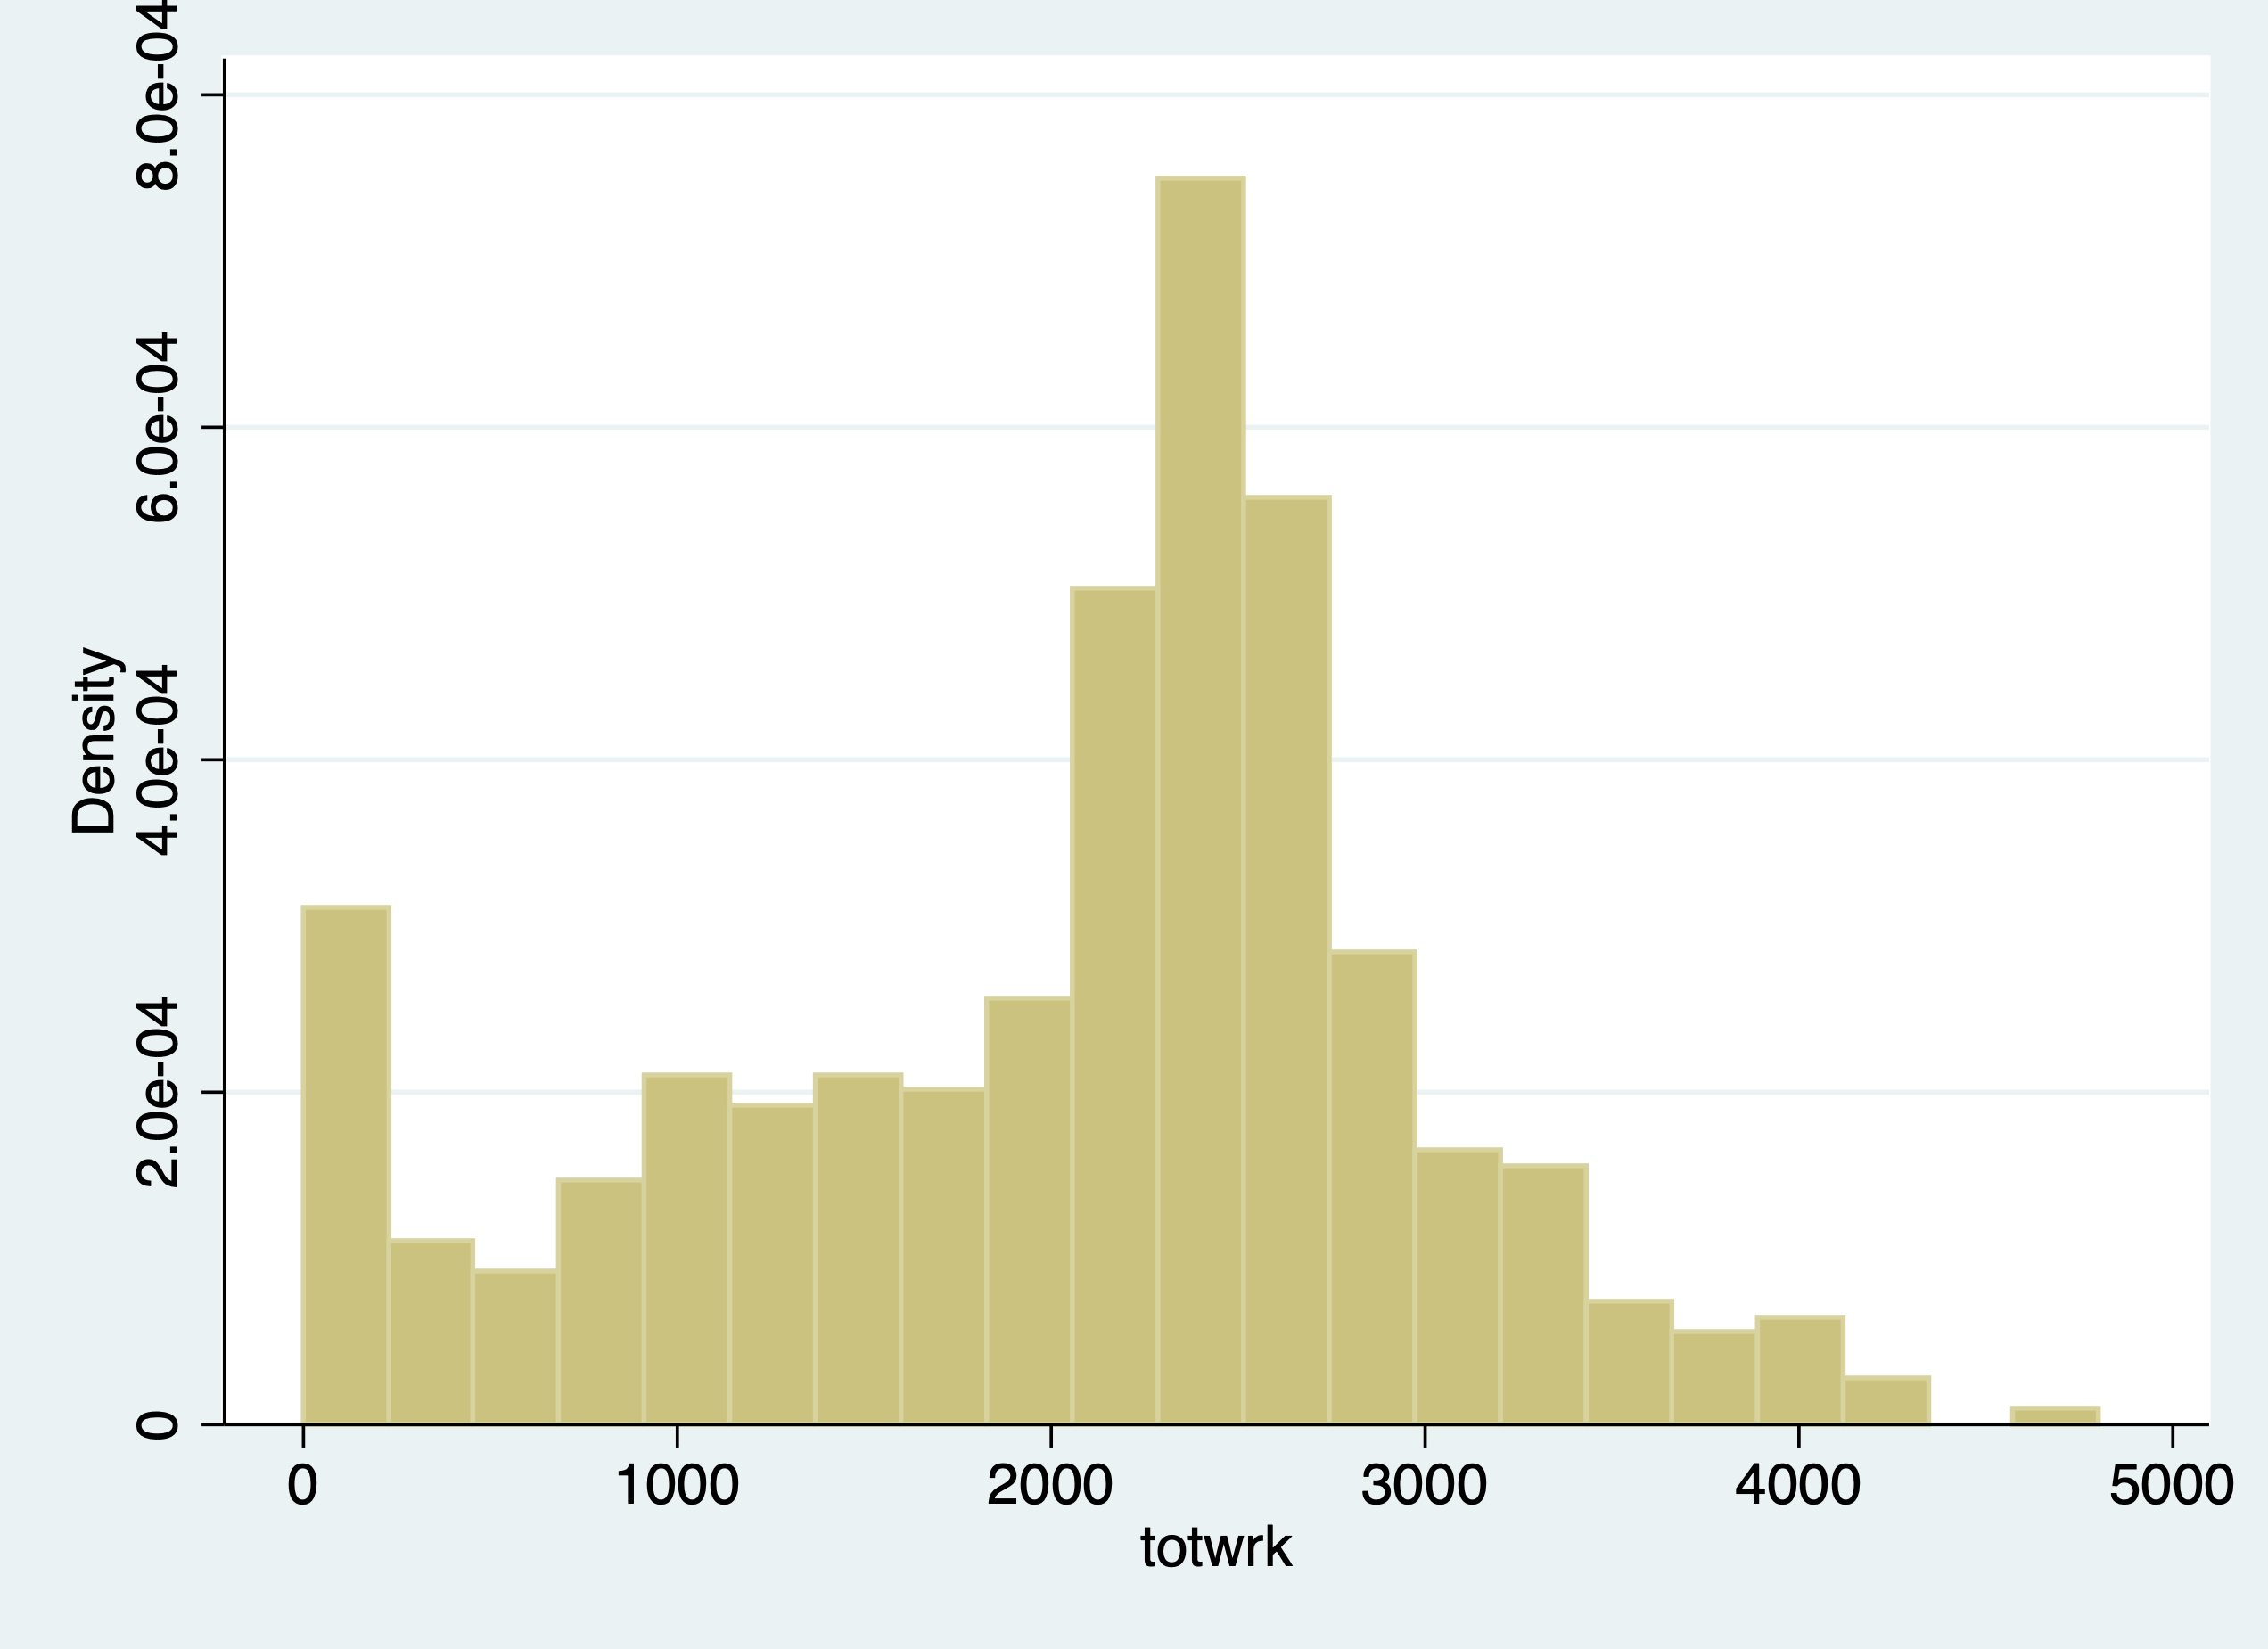
\includegraphics[keepaspectratio]{totwrk.png}}
\caption{Histogram of Annual Hours Worked}
\end{figure}

\begin{Shaded}
\begin{Highlighting}[]
\KeywordTok{histogram}\NormalTok{ slpnap}
\KeywordTok{graph} \KeywordTok{export} \StringTok{"/Users/Sam/Desktop/Econ 645/Stata/slpnap.png"}\NormalTok{, }\KeywordTok{replace}
\end{Highlighting}
\end{Shaded}

\begin{figure}
\centering
\pandocbounded{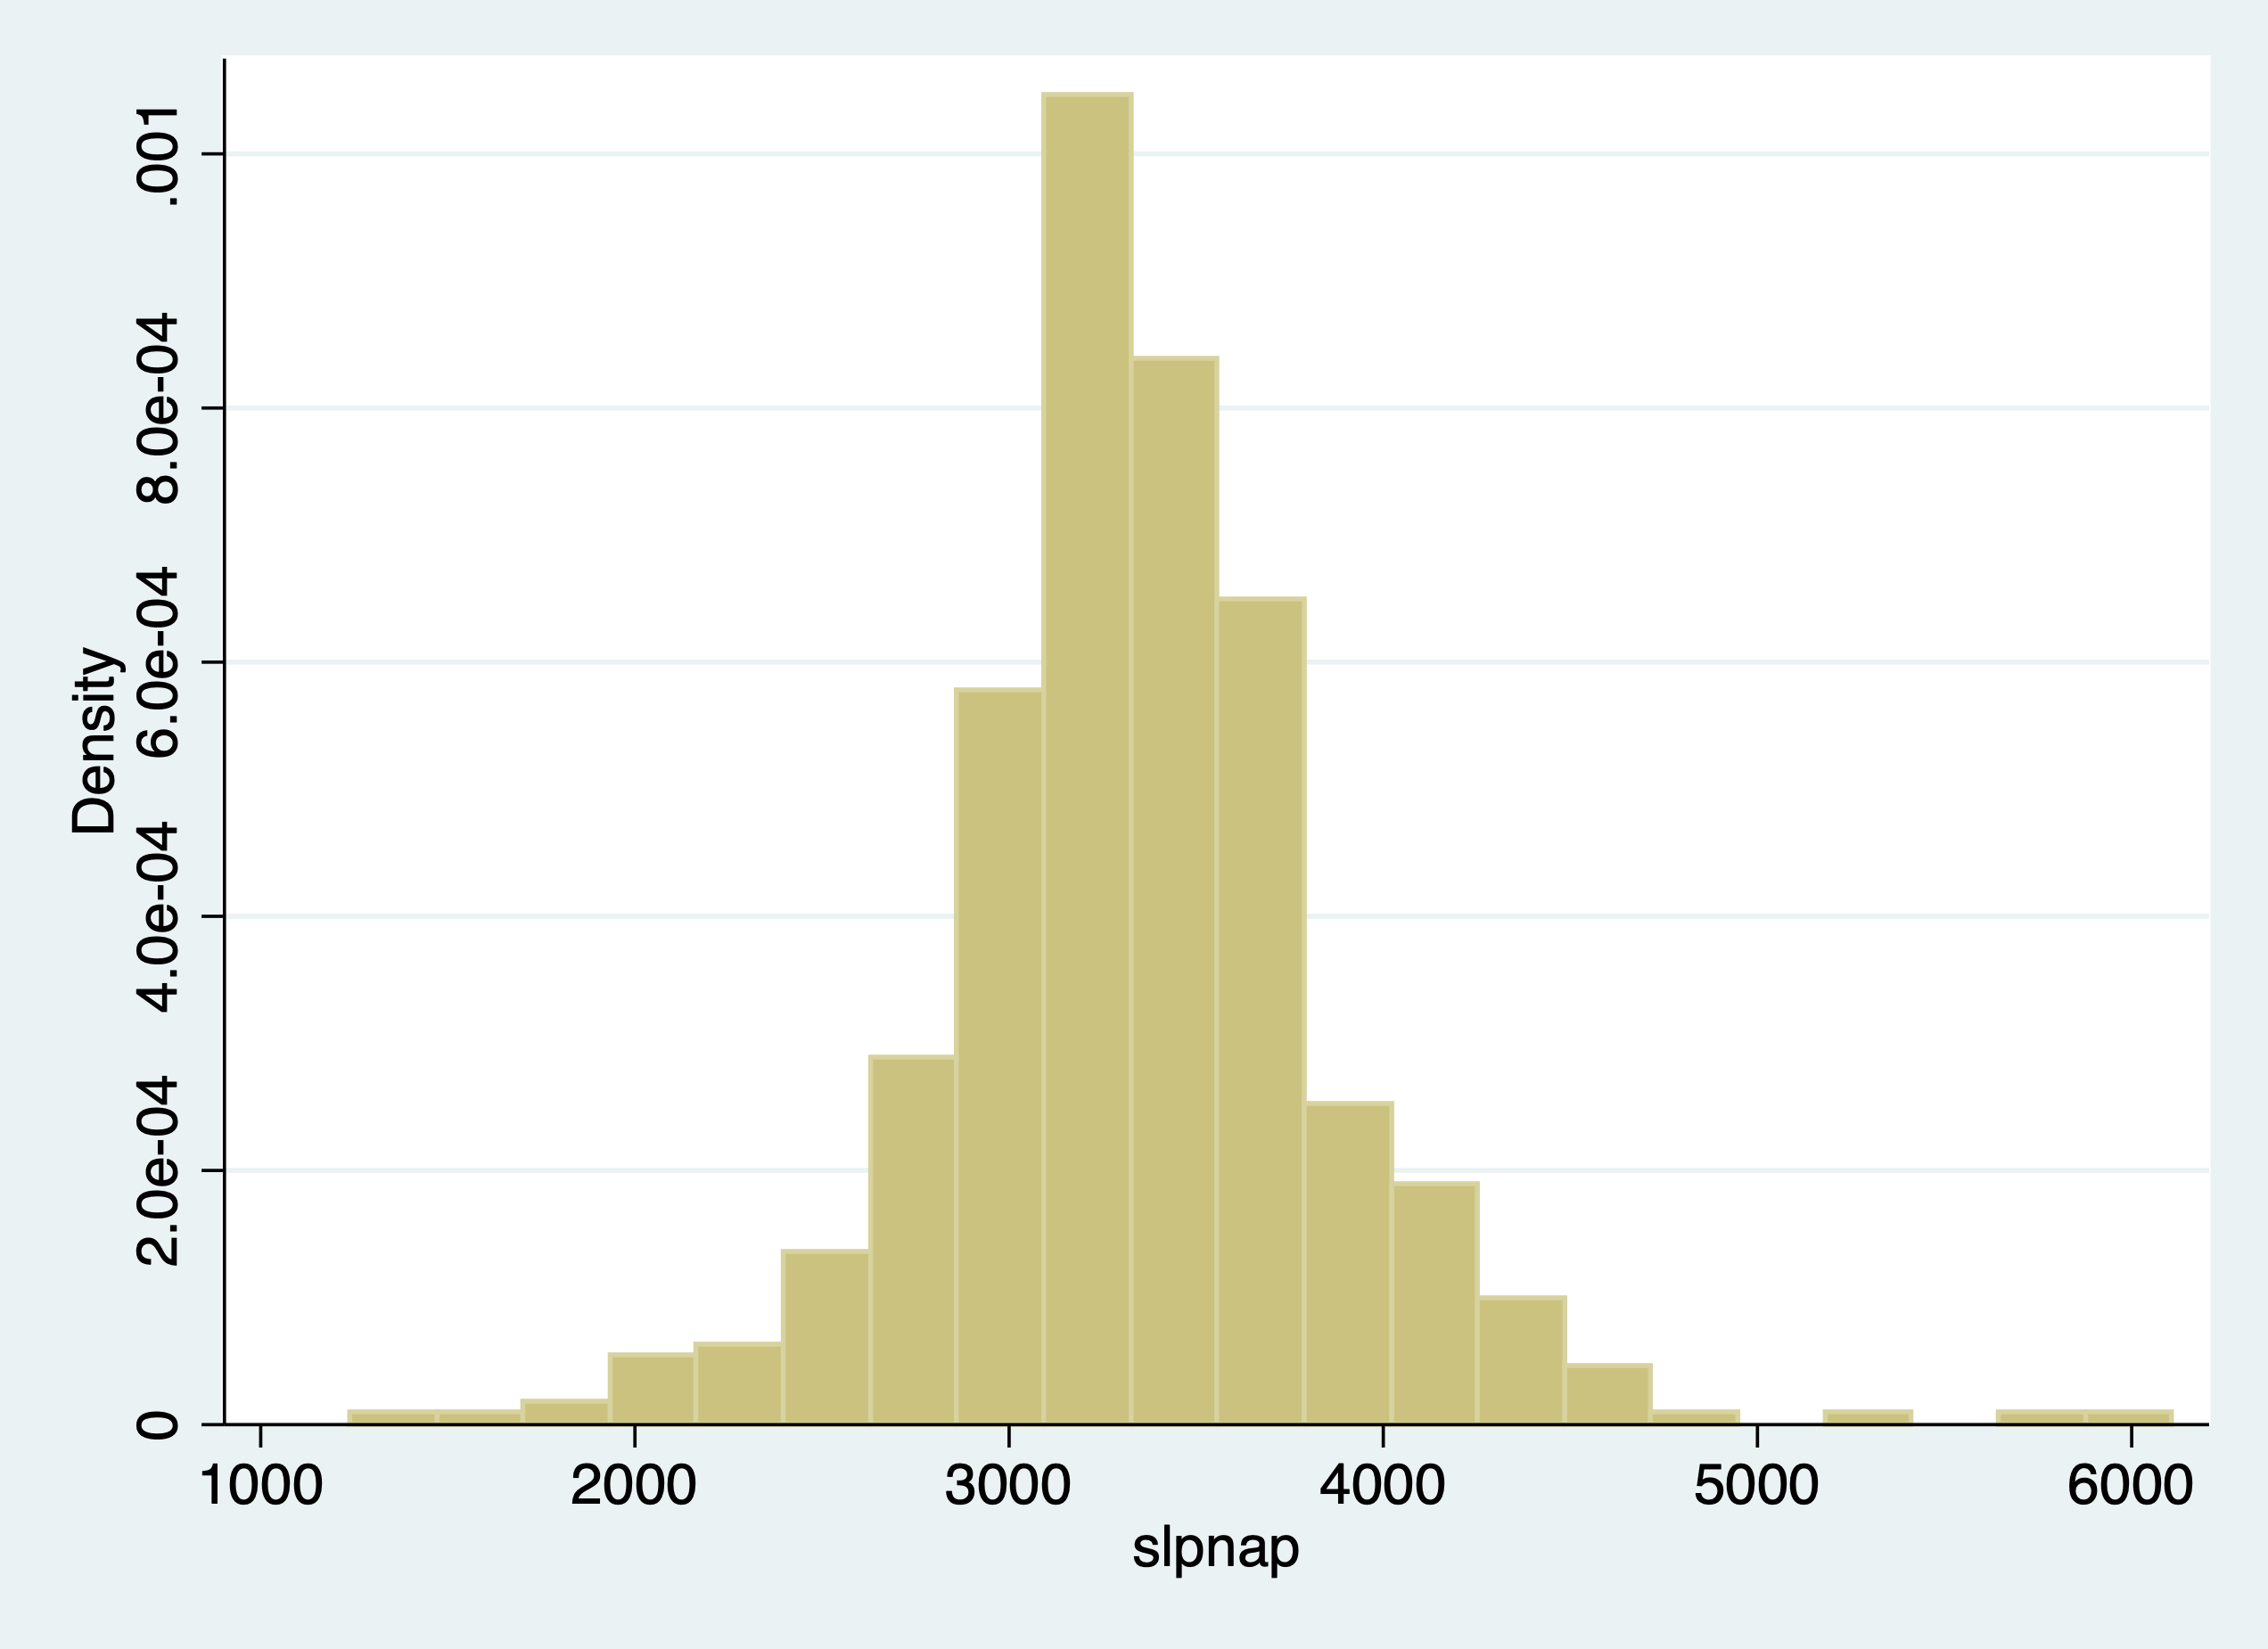
\includegraphics[keepaspectratio]{slpnap.png}}
\caption{Histogram of Minutes Sleeping Per Week}
\end{figure}

When we run OLS, we do not control for unobserved individual time-invariant effects.

Pooled OLS

\begin{Shaded}
\begin{Highlighting}[]
\KeywordTok{est} \KeywordTok{clear}
\NormalTok{eststo OLS: }\KeywordTok{reg}\NormalTok{ slpnap i.d81 totwrk educ marr yngkid gdhlth }
\end{Highlighting}
\end{Shaded}

\begin{verbatim}
      Source |       SS           df       MS      Number of obs   =       478
-------------+----------------------------------   F(6, 471)       =      8.50
       Model |  12812772.5         6  2135462.09   Prob > F        =    0.0000
    Residual |   118370944       471  251318.353   R-squared       =    0.0977
-------------+----------------------------------   Adj R-squared   =    0.0862
       Total |   131183717       477  275018.274   Root MSE        =    501.32

------------------------------------------------------------------------------
      slpnap |      Coef.   Std. Err.      t    P>|t|     [95% Conf. Interval]
-------------+----------------------------------------------------------------
       1.d81 |  -77.02965   47.96519    -1.61   0.109    -171.2819    17.22259
      totwrk |  -.1500954   .0244002    -6.15   0.000    -.1980421   -.1021487
        educ |  -20.25655   8.000179    -2.53   0.012    -35.97701   -4.536091
        marr |  -42.19389   53.07869    -0.79   0.427    -146.4942    62.10645
      yngkid |    74.2579   77.32582     0.96   0.337    -77.68838    226.2042
      gdhlth |   29.03733   59.57889     0.49   0.626    -88.03599    146.1107
       _cons |   3958.756   121.7663    32.51   0.000     3719.483    4198.028
------------------------------------------------------------------------------
\end{verbatim}

FD Model

\begin{Shaded}
\begin{Highlighting}[]
\NormalTok{eststo FD: }\KeywordTok{reg} \KeywordTok{d}\NormalTok{.slpnap }\KeywordTok{d}\NormalTok{.totwrk }\KeywordTok{d}\NormalTok{.educ }\KeywordTok{d}\NormalTok{.marr }\KeywordTok{d}\NormalTok{.yngkid }\KeywordTok{d}\NormalTok{.gdhlth}
\end{Highlighting}
\end{Shaded}

\begin{verbatim}
      Source |       SS           df       MS      Number of obs   =       239
-------------+----------------------------------   F(5, 233)       =      8.19
       Model |  14674698.2         5  2934939.64   Prob > F        =    0.0000
    Residual |  83482611.7       233  358294.471   R-squared       =    0.1495
-------------+----------------------------------   Adj R-squared   =    0.1313
       Total |  98157309.9       238  412425.672   Root MSE        =    598.58

------------------------------------------------------------------------------
    D.slpnap |      Coef.   Std. Err.      t    P>|t|     [95% Conf. Interval]
-------------+----------------------------------------------------------------
      totwrk |
         D1. |  -.2266694    .036054    -6.29   0.000    -.2977029   -.1556359
             |
        educ |
         D1. |  -.0244717   48.75938    -0.00   1.000    -96.09008    96.04113
             |
        marr |
         D1. |   104.2139   92.85536     1.12   0.263    -78.72946    287.1574
             |
      yngkid |
         D1. |    94.6654   87.65252     1.08   0.281    -78.02739    267.3582
             |
      gdhlth |
         D1. |   87.57785   76.59913     1.14   0.254    -63.33758    238.4933
             |
       _cons |  -92.63404    45.8659    -2.02   0.045    -182.9989   -2.269152
------------------------------------------------------------------------------
\end{verbatim}

Our Pooled OLS model shows one additional hour worked per year is associated with a 0.15 fewer minutes per week of sleep, while our FD model one additional hour worked per year is associated with a 0.23 fewer minutes of sleep per week.

Similar except time dummy and base intercepts look at the difference between educ in Pooled and FE models. There is likely a confounder between ability sleep and education.

\begin{Shaded}
\begin{Highlighting}[]
\NormalTok{esttab OLS FD, mtitles se scalars(}\FunctionTok{F}\NormalTok{ r2) }\KeywordTok{drop}\NormalTok{(0.d81)}
\end{Highlighting}
\end{Shaded}

\begin{verbatim}
                      (1)             (2)   
                      OLS              FD   
--------------------------------------------
1.d81              -77.03                   
                  (47.97)                   

totwrk             -0.150***                
                 (0.0244)                   

educ               -20.26*                  
                  (8.000)                   

marr               -42.19                   
                  (53.08)                   

yngkid              74.26                   
                  (77.33)                   

gdhlth              29.04                   
                  (59.58)                   

D.totwrk                           -0.227***
                                 (0.0361)   

D.educ                            -0.0245   
                                  (48.76)   

D.marr                              104.2   
                                  (92.86)   

D.yngkid                            94.67   
                                  (87.65)   

D.gdhlth                            87.58   
                                  (76.60)   

_cons              3958.8***       -92.63*  
                  (121.8)         (45.87)   
--------------------------------------------
N                     478             239   
F                   8.497           8.191   
r2                 0.0977           0.150   
--------------------------------------------
Standard errors in parentheses
* p<0.05, ** p<0.01, *** p<0.001
\end{verbatim}

Let's look at elasticities

\begin{Shaded}
\begin{Highlighting}[]
\KeywordTok{gen}\NormalTok{ lnslpnap=}\FunctionTok{ln}\NormalTok{(slpnap)}
\KeywordTok{gen}\NormalTok{ lntotwrk=}\FunctionTok{ln}\NormalTok{(totwrk)}
\KeywordTok{gen}\NormalTok{ lneduc=}\FunctionTok{ln}\NormalTok{(educ)}
\end{Highlighting}
\end{Shaded}

FD Model

\begin{Shaded}
\begin{Highlighting}[]
\KeywordTok{reg} \KeywordTok{d}\NormalTok{.lnslpnap }\KeywordTok{d}\NormalTok{.lntotwrk }\KeywordTok{d}\NormalTok{.lneduc }\KeywordTok{d}\NormalTok{.marr }\KeywordTok{d}\NormalTok{.yngkid }\KeywordTok{d}\NormalTok{.gdhlth}
\end{Highlighting}
\end{Shaded}

\begin{verbatim}
      Source |       SS           df       MS      Number of obs   =       214
-------------+----------------------------------   F(5, 208)       =      4.17
       Model |  .805249181         5  .161049836   Prob > F        =    0.0012
    Residual |  8.03583239       208   .03863381   R-squared       =    0.0911
-------------+----------------------------------   Adj R-squared   =    0.0692
       Total |  8.84108157       213  .041507425   Root MSE        =    .19655

------------------------------------------------------------------------------
  D.lnslpnap |      Coef.   Std. Err.      t    P>|t|     [95% Conf. Interval]
-------------+----------------------------------------------------------------
    lntotwrk |
         D1. |  -.0848256   .0206499    -4.11   0.000    -.1255354   -.0441158
             |
      lneduc |
         D1. |  -.0289507   .2628724    -0.11   0.912    -.5471864     .489285
             |
        marr |
         D1. |  -.0038529   .0323002    -0.12   0.905    -.0675306    .0598247
             |
      yngkid |
         D1. |   .0056761   .0290466     0.20   0.845    -.0515874    .0629397
             |
      gdhlth |
         D1. |    .048008   .0266772     1.80   0.073    -.0045843    .1006004
             |
       _cons |  -.0204204   .0155593    -1.31   0.191    -.0510947    .0102538
------------------------------------------------------------------------------
\end{verbatim}

A 1\% increase in hours worked per year is associated with a 0.08\% decrease in sleep per week.

\subsection{Distributed Lag of Crime Rates on Clear-up Rate}\label{distributed-lag-of-crime-rates-on-clear-up-rate}

\textbf{Lesson:} Lagged variables can be important explanatory variables
\emph{Note:} We'll get into this a bit more in Wooldridge Chapter 10-12.

We will get into time series later in the course, but we will have a preview. With panel data, we are able to see the same observation over time. Given this, we can see if lagged values affect current values for the cross-sectional unit of observation.

Eide(1994) wants to assess if prior clear-up rates for crime have a relationship with crime rates in the current time period. The dependent variable of interest is the current period crime rate. The variable of interest is the clear-up percentage which is the rate of crimes that have lead to conviction.

We will use a log-log model and use a first-difference.

\[ \Delta ln(crime_{i,t}= \delta_0 + \beta_1 \Delta ln(clearup_{i,t-1}) + \beta_2 \Delta ln(clearup_{i,t-2}) + \Delta \varepsilon_{i,t} \]

\begin{Shaded}
\begin{Highlighting}[]
\NormalTok{cd }\StringTok{"/Users/Sam/Desktop/Econ 645/Data/Wooldridge"}
\KeywordTok{use}\NormalTok{ crime3.dta, }\KeywordTok{clear}
\KeywordTok{reg}\NormalTok{ clcrime cclrprc1 cclrprc2}
\end{Highlighting}
\end{Shaded}

\begin{verbatim}
/Users/Sam/Desktop/Econ 645/Data/Wooldridge

      Source |       SS           df       MS      Number of obs   =        53
-------------+----------------------------------   F(2, 50)        =      5.99
       Model |  1.42294697         2  .711473484   Prob > F        =    0.0046
    Residual |  5.93723904        50  .118744781   R-squared       =    0.1933
-------------+----------------------------------   Adj R-squared   =    0.1611
       Total |  7.36018601        52  .141542039   Root MSE        =    .34459

------------------------------------------------------------------------------
     clcrime |      Coef.   Std. Err.      t    P>|t|     [95% Conf. Interval]
-------------+----------------------------------------------------------------
    cclrprc1 |  -.0040475   .0047199    -0.86   0.395    -.0135276    .0054326
    cclrprc2 |  -.0131966   .0051946    -2.54   0.014    -.0236302   -.0027629
       _cons |   .0856556   .0637825     1.34   0.185    -.0424553    .2137665
------------------------------------------------------------------------------
\end{verbatim}

Our model tells us that 1 percent increase in getting crimes to conviction leads to a reduction in the current period crime rate of about 1.32 percent. Assuming this model is specified well, crime rates are sensitive to clear-up rates from the prior 2 years.

\subsection{Enterprise Zones and Unemployment}\label{enterprise-zones-and-unemployment}

\textbf{Lesson:} We need to be aware of heteroskedasticity and serial correlation

We should test for heteroskedasticity and serial correlation when running our First-Difference Estimator.

Serial correlation means that the differences in the idiosyncractic errors between time periods are correlated, which is a violation of our assumption that there is no serial correlation for our first-difference estimator.

We'll use data from Papke (1994) who studied the effect of Indiana's enterprise zone program on unemployment claims. Do enterprise zones increase employment and reduce unemployment claims?

She analyzes 22 cities in Indiana from 1980 to 1988, since 6 enterprise zones were established in 1984. Twelve cities did not receive the enterprise zones, while 10 cities did get enterprise zones.

We'll use a simple analysis that the change in natural log of unemployment
claims is a function of time period binaries, change in enterprise zones, and
the idiosyncractic error.

One way to do it is to use the data already created.

\[ ln(UnempClaims_{i,t}) = \beta_0 + \beta_1 EnterpriseZone_{i,t} + a_t + a_i + \varepsilon_{i,t} \]

Pooled OLS

\begin{Shaded}
\begin{Highlighting}[]
\NormalTok{cd }\StringTok{"/Users/Sam/Desktop/Econ 645/Data/Wooldridge"}
\KeywordTok{use} \StringTok{"ezunem.dta"}\NormalTok{, }\KeywordTok{clear}
\KeywordTok{reg}\NormalTok{ luclms i.d82 i.d83 i.d84 i.d85 i.d86 i.d87 i.d88 cez}
\end{Highlighting}
\end{Shaded}

\begin{verbatim}
/Users/Sam/Desktop/Econ 645/Data/Wooldridge

      Source |       SS           df       MS      Number of obs   =       176
-------------+----------------------------------   F(8, 167)       =     10.39
       Model |  29.2551235         8  3.65689043   Prob > F        =    0.0000
    Residual |  58.7753327       167    .3519481   R-squared       =    0.3323
-------------+----------------------------------   Adj R-squared   =    0.3003
       Total |  88.0304561       175  .503031178   Root MSE        =    .59325

------------------------------------------------------------------------------
      luclms |      Coef.   Std. Err.      t    P>|t|     [95% Conf. Interval]
-------------+----------------------------------------------------------------
       1.d82 |   .4571276   .1788722     2.56   0.011     .1039853    .8102699
       1.d83 |   .1023765   .1788722     0.57   0.568    -.2507658    .4555188
       1.d84 |  -.2821805   .1882109    -1.50   0.136    -.6537598    .0893988
       1.d85 |  -.3150721   .1830816    -1.72   0.087    -.6765248    .0463805
       1.d86 |  -.3470941   .1788722    -1.94   0.054    -.7002364    .0060481
       1.d87 |   -.614778   .1788722    -3.44   0.001    -.9679202   -.2616357
       1.d88 |  -.9534624   .1788722    -5.33   0.000    -1.306605   -.6003201
         cez |  -.0139924   .2146822    -0.07   0.948    -.4378332    .4098484
       _cons |   11.37276   .1264818    89.92   0.000     11.12305    11.62247
------------------------------------------------------------------------------
\end{verbatim}

Let's say we didn't have the data already created. What we'll need to do
is to set the panel data with xtset unit timeperiod
Set the Panel Data

\begin{Shaded}
\begin{Highlighting}[]
\NormalTok{xtset city }\FunctionTok{year}
\end{Highlighting}
\end{Shaded}

\begin{verbatim}
       panel variable:  city (strongly balanced)
        time variable:  year, 1980 to 1988
                delta:  1 unit
\end{verbatim}

We can use the \emph{d.} operator to use a first difference
First Difference

\begin{Shaded}
\begin{Highlighting}[]
\KeywordTok{reg} \KeywordTok{d}\NormalTok{.luclms i.d82 i.d83 i.d84 i.d85 i.d86 i.d87 i.d88 }\KeywordTok{d}\NormalTok{.ez}
\end{Highlighting}
\end{Shaded}

\begin{verbatim}
      Source |       SS           df       MS      Number of obs   =       176
-------------+----------------------------------   F(8, 167)       =     34.50
       Model |  12.8826331         8  1.61032914   Prob > F        =    0.0000
    Residual |  7.79583815       167  .046681666   R-squared       =    0.6230
-------------+----------------------------------   Adj R-squared   =    0.6049
       Total |  20.6784713       175  .118162693   Root MSE        =    .21606

------------------------------------------------------------------------------
    D.luclms |      Coef.   Std. Err.      t    P>|t|     [95% Conf. Interval]
-------------+----------------------------------------------------------------
       1.d82 |   .7787595   .0651444    11.95   0.000     .6501469    .9073721
       1.d83 |  -.0331192   .0651444    -0.51   0.612    -.1617318    .0954934
       1.d84 |  -.0171382   .0685455    -0.25   0.803    -.1524655    .1181891
       1.d85 |    .323081   .0666774     4.85   0.000     .1914417    .4547202
       1.d86 |    .292154   .0651444     4.48   0.000     .1635413    .4207666
       1.d87 |   .0539481   .0651444     0.83   0.409    -.0746645    .1825607
       1.d88 |  -.0170526   .0651444    -0.26   0.794    -.1456652    .1115601
             |
          ez |
         D1. |  -.1818775   .0781862    -2.33   0.021    -.3362382   -.0275169
             |
       _cons |  -.3216319    .046064    -6.98   0.000    -.4125748   -.2306891
------------------------------------------------------------------------------
\end{verbatim}

Test for Heteroskedasticity:

Bruesch-Pagan/Cameron-Trivedi Test using \emph{estat} post-estimation command

\begin{Shaded}
\begin{Highlighting}[]
\KeywordTok{estat} \KeywordTok{imtest}
\end{Highlighting}
\end{Shaded}

\begin{verbatim}
Cameron & Trivedi's decomposition of IM-test

---------------------------------------------------
              Source |       chi2     df      p
---------------------+-----------------------------
  Heteroskedasticity |      12.85      9    0.1697
            Skewness |      13.04      8    0.1104
            Kurtosis |       0.11      1    0.7414
---------------------+-----------------------------
               Total |      26.00     18    0.0998
---------------------------------------------------
\end{verbatim}

White Test using \emph{estat} postestimation command

\begin{Shaded}
\begin{Highlighting}[]
\KeywordTok{estat} \KeywordTok{imtest}\NormalTok{, }\BaseNTok{white}
\end{Highlighting}
\end{Shaded}

\begin{verbatim}
White's test for Ho: homoskedasticity
         against Ha: unrestricted heteroskedasticity

         chi2(9)      =     12.85
         Prob > chi2  =    0.1697

Cameron & Trivedi's decomposition of IM-test

---------------------------------------------------
              Source |       chi2     df      p
---------------------+-----------------------------
  Heteroskedasticity |      12.85      9    0.1697
            Skewness |      13.04      8    0.1104
            Kurtosis |       0.11      1    0.7414
---------------------+-----------------------------
               Total |      26.00     18    0.0998
---------------------------------------------------
\end{verbatim}

We fail to reject the null hypothesis of homoskedastic standard errors.

Test for autocorrelation
We can use the command xtserial to test for serial correlation, since we already
set up our panel above.

\begin{Shaded}
\begin{Highlighting}[]
    \KeywordTok{help}\NormalTok{ xtserial}
\end{Highlighting}
\end{Shaded}

\begin{Shaded}
\begin{Highlighting}[]
\NormalTok{xtserial luclms d83 d84 d85 d86 d87 d88 cez, output}
\end{Highlighting}
\end{Shaded}

\begin{verbatim}
Linear regression                               Number of obs     =        154
                                                F(7, 21)          =     102.85
                                                Prob > F          =     0.0000
                                                R-squared         =     0.4711
                                                Root MSE          =     .28063

                                  (Std. Err. adjusted for 22 clusters in city)
------------------------------------------------------------------------------
             |               Robust
    D.luclms |      Coef.   Std. Err.      t    P>|t|     [95% Conf. Interval]
-------------+----------------------------------------------------------------
         d83 |
         D1. |  -.3547511   .0410541    -8.64   0.000    -.4401277   -.2693745
             |
         d84 |
         D1. |  -.7240107   .0816269    -8.87   0.000     -.893763   -.5542583
             |
         d85 |
         D1. |  -.7620015   .0540757   -14.09   0.000    -.8744581   -.6495448
             |
         d86 |
         D1. |  -.8042218   .0490039   -16.41   0.000     -.906131   -.7023126
             |
         d87 |
         D1. |  -1.071906   .0496977   -21.57   0.000    -1.175258   -.9685535
             |
         d88 |
         D1. |   -1.41059    .065833   -21.43   0.000    -1.547497   -1.273683
             |
         cez |
         D1. |   -.070083   .0650804    -1.08   0.294     -.205425     .065259
------------------------------------------------------------------------------

Wooldridge test for autocorrelation in panel data
H0: no first-order autocorrelation
    F(  1,      21) =    120.981
           Prob > F =      0.0000
\end{verbatim}

We reject the null hypothesis that the differences in idiosyncratic errors is 0.

What can we do for this serial correlation? We can cluster our standard errors to account for the serial correlation within units.

Robust for serial correlation within unit of analysis clusters

\begin{Shaded}
\begin{Highlighting}[]
\KeywordTok{reg} \KeywordTok{d}\NormalTok{.luclms i.d82 i.d83 i.d84 i.d85 i.d86 i.d87 i.d88 }\KeywordTok{d}\NormalTok{.cez, }\KeywordTok{robust} \KeywordTok{cluster}\NormalTok{(city)}
\end{Highlighting}
\end{Shaded}

\begin{verbatim}
note: 1.d88 omitted because of collinearity

Linear regression                               Number of obs     =        154
                                                F(7, 21)          =      41.20
                                                Prob > F          =     0.0000
                                                R-squared         =     0.6333
                                                Root MSE          =     .21865

                                  (Std. Err. adjusted for 22 clusters in city)
------------------------------------------------------------------------------
             |               Robust
    D.luclms |      Coef.   Std. Err.      t    P>|t|     [95% Conf. Interval]
-------------+----------------------------------------------------------------
       1.d82 |   .7958121   .0577076    13.79   0.000     .6758025    .9158217
       1.d83 |  -.0160666   .0565946    -0.28   0.779    -.1337615    .1016282
       1.d84 |  -.0305751   .0742049    -0.41   0.684    -.1848926    .1237424
       1.d85 |   .3006937   .0568959     5.28   0.000     .1823723    .4190151
       1.d86 |   .2964642   .0786548     3.77   0.001     .1328926    .4600357
       1.d87 |   .0710007   .0462206     1.54   0.139    -.0251204    .1671217
       1.d88 |          0  (omitted)
             |
         cez |
         D1. |   -.070083   .0653029    -1.07   0.295    -.2058877    .0657217
             |
       _cons |  -.3386845   .0359416    -9.42   0.000    -.4134292   -.2639397
------------------------------------------------------------------------------
\end{verbatim}

Once we account for the serial correlation in the idiosyncratic error, our coefficient on the change in enterprise zone becomes statistically insignificant.

Testing for serial correlation, and Clustering your standard error at the treatment level is an important test and step with FD estimators.

When we get to Fixed Effects (Within) estimator, the assumption is slightly different. For First-Difference Estimator, the DIFFERENCE in idiosyncratic errors cannot be correlated, but for Fixed-Effects (Within) Estimator the assumption states that only the idiosyncratic errors cannot be correlated.

\subsection{County Crimes in North Carolina}\label{county-crimes-in-north-carolina}

\textbf{Lesson:} First-Difference Estimator (and Fixed Effects Estimator) cannot fix simultaneity bias. We need an valid instrument to deal with simultaneity bias.

Cornwell and Trumbull (1994) analyzed data on 90 counties in North Carolina from 1981 to 1987 to using panel data to account for time-invariant effects. Their cross-sectional unit of observation is the county (not individuals within a county). They want to know what the is the effect of police per capita on crime rates.

For our model the dependent variable is the change in the natural log of crimes per person (lcrimrte). They are interested in estimating the sensitivity of police per capita (polpc) on crime rate, so they use the difference in natural log of police per capita. This will get you elasticities, which provide useful interpretations of percentage increases.

They also control for the difference in natural log of probability of arrest (prbarr), the probability of conviction (prbconv), the probability of serving time in prison given a conviction (prbpris), and the average sentence length.

\[ ln(crimerate_{i,t}) = \beta_0 + \beta_1 ln(prbcon_{i,t}) + \beta_2 ln(prbpris_{i,t}) + \beta_3 ln(avgsen_{i,t}) + \beta_4 ln(polpc_{i,t}) + a_t + a_i + \varepsilon_{i,t} \]
Pooled OLS

\begin{Shaded}
\begin{Highlighting}[]
\NormalTok{cd }\StringTok{"/Users/Sam/Desktop/Econ 645/Data/Wooldridge"}
\KeywordTok{use} \StringTok{"crime4.dta"}\NormalTok{, }\KeywordTok{clear}
\KeywordTok{reg}\NormalTok{ lcrmrte i.d82 i.d83 i.d84 i.d85 i.d86 i.d87 lprbarr lprbconv lprbpris lavgsen lpolpc}
\end{Highlighting}
\end{Shaded}

\begin{verbatim}
/Users/Sam/Desktop/Econ 645/Data/Wooldridge

      Source |       SS           df       MS      Number of obs   =       630
-------------+----------------------------------   F(11, 618)      =     74.49
       Model |  117.644669        11  10.6949699   Prob > F        =    0.0000
    Residual |   88.735673       618  .143585231   R-squared       =    0.5700
-------------+----------------------------------   Adj R-squared   =    0.5624
       Total |  206.380342       629  .328108652   Root MSE        =    .37893

------------------------------------------------------------------------------
     lcrmrte |      Coef.   Std. Err.      t    P>|t|     [95% Conf. Interval]
-------------+----------------------------------------------------------------
       1.d82 |   .0051371    .057931     0.09   0.929    -.1086284    .1189026
       1.d83 |   -.043503   .0576243    -0.75   0.451    -.1566662    .0696601
       1.d84 |  -.1087542    .057923    -1.88   0.061     -.222504    .0049957
       1.d85 |  -.0780454   .0583244    -1.34   0.181    -.1925835    .0364928
       1.d86 |  -.0420791   .0578218    -0.73   0.467      -.15563    .0714719
       1.d87 |  -.0270426    .056899    -0.48   0.635    -.1387815    .0846963
     lprbarr |  -.7195033   .0367657   -19.57   0.000    -.7917042   -.6473024
    lprbconv |  -.5456589   .0263683   -20.69   0.000    -.5974413   -.4938765
    lprbpris |   .2475521   .0672268     3.68   0.000     .1155314    .3795728
     lavgsen |  -.0867575   .0579205    -1.50   0.135    -.2005023    .0269872
      lpolpc |   .3659886   .0300252    12.19   0.000     .3070248    .4249525
       _cons |  -2.082293   .2516253    -8.28   0.000    -2.576438   -1.588149
------------------------------------------------------------------------------
\end{verbatim}

First Difference

\begin{Shaded}
\begin{Highlighting}[]
\NormalTok{xtset county }\FunctionTok{year}
\end{Highlighting}
\end{Shaded}

\begin{verbatim}
       panel variable:  county (strongly balanced)
        time variable:  year, 81 to 87
                delta:  1 unit
\end{verbatim}

With xtset, we can use the d.~for our explanatory variables.

First-Difference

\begin{Shaded}
\begin{Highlighting}[]
\KeywordTok{reg} \KeywordTok{d}\NormalTok{.lcrmrte i.d83 i.d84 i.d85 i.d86 i.d87 }\KeywordTok{d}\NormalTok{.lprbarr }\KeywordTok{d}\NormalTok{.lprbconv }\KeywordTok{d}\NormalTok{.lprbpris }\KeywordTok{d}\NormalTok{.lavgsen }\KeywordTok{d}\NormalTok{.lpolpc}
\end{Highlighting}
\end{Shaded}

\begin{verbatim}
      Source |       SS           df       MS      Number of obs   =       540
-------------+----------------------------------   F(10, 529)      =     40.32
       Model |  9.60042828        10  .960042828   Prob > F        =    0.0000
    Residual |  12.5963755       529  .023811674   R-squared       =    0.4325
-------------+----------------------------------   Adj R-squared   =    0.4218
       Total |  22.1968038       539  .041181454   Root MSE        =    .15431

------------------------------------------------------------------------------
   D.lcrmrte |      Coef.   Std. Err.      t    P>|t|     [95% Conf. Interval]
-------------+----------------------------------------------------------------
       1.d83 |  -.0998658   .0238953    -4.18   0.000    -.1468071   -.0529246
       1.d84 |  -.0479374   .0235021    -2.04   0.042    -.0941063   -.0017686
       1.d85 |  -.0046111   .0234998    -0.20   0.845    -.0507756    .0415533
       1.d86 |   .0275143   .0241494     1.14   0.255    -.0199261    .0749548
       1.d87 |   .0408267   .0244153     1.67   0.095    -.0071361    .0887895
             |
     lprbarr |
         D1. |  -.3274942   .0299801   -10.92   0.000    -.3863889   -.2685994
             |
    lprbconv |
         D1. |  -.2381066   .0182341   -13.06   0.000    -.2739268   -.2022864
             |
    lprbpris |
         D1. |  -.1650462    .025969    -6.36   0.000    -.2160613   -.1140312
             |
     lavgsen |
         D1. |  -.0217607   .0220909    -0.99   0.325    -.0651574     .021636
             |
      lpolpc |
         D1. |   .3984264    .026882    14.82   0.000     .3456177     .451235
             |
       _cons |   .0077134   .0170579     0.45   0.651    -.0257961    .0412229
------------------------------------------------------------------------------
\end{verbatim}

So our model is estimating that a 1\% increase in police per capita increases the crime rate by about 0.4\%. We would expect that increases in police per capita would reduce crime rates. This is likely shows that there are problems in our model.

What is happening? Likely simultaneity bias is occurring. Areas with high crime rates have more police per capita, which more police per capita is associated with higher crime rates. It's a circular/endogenous reference, so we will need an valid instrument to deal with this simultaneity bias/endogeneity.

We can test for heteroskedasticity and serial correlation, but this only affects our standard errors, not our coefficients.

Test for autocorrelation with one lag AR(1). We can see that serial correlation is a problem, which means we should cluster our standard errors at the county level.

\begin{Shaded}
\begin{Highlighting}[]
\KeywordTok{predict} \FunctionTok{r}\NormalTok{, residual}
\KeywordTok{gen}\NormalTok{ lag\_r =}\OtherTok{l}\NormalTok{.}\FunctionTok{r}
\KeywordTok{reg} \FunctionTok{r}\NormalTok{ lag\_r i.d83 i.d84 i.d85 i.d86 i.d87 }\KeywordTok{d}\NormalTok{.lprbarr }\KeywordTok{d}\NormalTok{.lprbconv }\KeywordTok{d}\NormalTok{.lprbpris }\KeywordTok{d}\NormalTok{.lavgsen }\KeywordTok{d}\NormalTok{.lpolpc}
\end{Highlighting}
\end{Shaded}

\begin{verbatim}
(90 missing values generated)

(180 missing values generated)

note: 1.d87 omitted because of collinearity

      Source |       SS           df       MS      Number of obs   =       450
-------------+----------------------------------   F(10, 439)      =      2.35
       Model |  .564663971        10  .056466397   Prob > F        =    0.0102
    Residual |   10.528838       439  .023983686   R-squared       =    0.0509
-------------+----------------------------------   Adj R-squared   =    0.0293
       Total |   11.093502       449  .024707131   Root MSE        =    .15487

------------------------------------------------------------------------------
           r |      Coef.   Std. Err.      t    P>|t|     [95% Conf. Interval]
-------------+----------------------------------------------------------------
       lag_r |  -.2332117   .0488802    -4.77   0.000      -.32928   -.1371435
       1.d83 |  -.0012379   .0234019    -0.05   0.958    -.0472317    .0447558
       1.d84 |  -.0016543   .0236303    -0.07   0.944    -.0480968    .0447883
       1.d85 |  -.0006044   .0236114    -0.03   0.980    -.0470098    .0458009
       1.d86 |   .0008841   .0233216     0.04   0.970    -.0449517    .0467199
       1.d87 |          0  (omitted)
             |
     lprbarr |
         D1. |   .0082875   .0330698     0.25   0.802    -.0567074    .0732823
             |
    lprbconv |
         D1. |  -.0036161   .0200155    -0.18   0.857    -.0429542    .0357221
             |
    lprbpris |
         D1. |   .0017131    .027855     0.06   0.951    -.0530326    .0564588
             |
     lavgsen |
         D1. |  -.0125831   .0245006    -0.51   0.608    -.0607362      .03557
             |
      lpolpc |
         D1. |   .0214883   .0282688     0.76   0.448    -.0340706    .0770473
             |
       _cons |   .0005347   .0167411     0.03   0.975     -.032368    .0334373
------------------------------------------------------------------------------
\end{verbatim}

We can always use our xtserial command to test for AR(1) serial correlation.

\begin{Shaded}
\begin{Highlighting}[]
\KeywordTok{reg} \KeywordTok{d}\NormalTok{.lcrmrte i.d83 i.d84 i.d85 i.d86 i.d87 }\KeywordTok{d}\NormalTok{.lprbarr }\KeywordTok{d}\NormalTok{.lprbconv }\KeywordTok{d}\NormalTok{.lprbpris }\KeywordTok{d}\NormalTok{.lavgsen }\KeywordTok{d}\NormalTok{.lpolpc}
\NormalTok{xtserial lcrmrte d83 d84 d85 d86 d87 lprbarr lprbconv lprbpris lavgsen lpolpc, output}
\end{Highlighting}
\end{Shaded}

\begin{verbatim}
      Source |       SS           df       MS      Number of obs   =       540
-------------+----------------------------------   F(10, 529)      =     40.32
       Model |  9.60042828        10  .960042828   Prob > F        =    0.0000
    Residual |  12.5963755       529  .023811674   R-squared       =    0.4325
-------------+----------------------------------   Adj R-squared   =    0.4218
       Total |  22.1968038       539  .041181454   Root MSE        =    .15431

------------------------------------------------------------------------------
   D.lcrmrte |      Coef.   Std. Err.      t    P>|t|     [95% Conf. Interval]
-------------+----------------------------------------------------------------
       1.d83 |  -.0998658   .0238953    -4.18   0.000    -.1468071   -.0529246
       1.d84 |  -.0479374   .0235021    -2.04   0.042    -.0941063   -.0017686
       1.d85 |  -.0046111   .0234998    -0.20   0.845    -.0507756    .0415533
       1.d86 |   .0275143   .0241494     1.14   0.255    -.0199261    .0749548
       1.d87 |   .0408267   .0244153     1.67   0.095    -.0071361    .0887895
             |
     lprbarr |
         D1. |  -.3274942   .0299801   -10.92   0.000    -.3863889   -.2685994
             |
    lprbconv |
         D1. |  -.2381066   .0182341   -13.06   0.000    -.2739268   -.2022864
             |
    lprbpris |
         D1. |  -.1650462    .025969    -6.36   0.000    -.2160613   -.1140312
             |
     lavgsen |
         D1. |  -.0217607   .0220909    -0.99   0.325    -.0651574     .021636
             |
      lpolpc |
         D1. |   .3984264    .026882    14.82   0.000     .3456177     .451235
             |
       _cons |   .0077134   .0170579     0.45   0.651    -.0257961    .0412229
------------------------------------------------------------------------------


Linear regression                               Number of obs     =        540
                                                F(10, 89)         =      13.68
                                                Prob > F          =     0.0000
                                                R-squared         =     0.4323
                                                Root MSE          =     .15419

                                (Std. Err. adjusted for 90 clusters in county)
------------------------------------------------------------------------------
             |               Robust
   D.lcrmrte |      Coef.   Std. Err.      t    P>|t|     [95% Conf. Interval]
-------------+----------------------------------------------------------------
         d83 |
         D1. |  -.0920147   .0146354    -6.29   0.000     -.121095   -.0629345
             |
         d84 |
         D1. |  -.1323557   .0179759    -7.36   0.000    -.1680734    -.096638
             |
         d85 |
         D1. |  -.1293278   .0232716    -5.56   0.000    -.1755679   -.0830876
             |
         d86 |
         D1. |  -.0938692   .0209561    -4.48   0.000    -.1355086   -.0522298
             |
         d87 |
         D1. |  -.0449434   .0236533    -1.90   0.061     -.091942    .0020552
             |
     lprbarr |
         D1. |  -.3263268   .0561808    -5.81   0.000     -.437957   -.2146967
             |
    lprbconv |
         D1. |  -.2375214   .0392585    -6.05   0.000    -.3155272   -.1595155
             |
    lprbpris |
         D1. |  -.1645109   .0457092    -3.60   0.001     -.255334   -.0736878
             |
     lavgsen |
         D1. |  -.0246909   .0252756    -0.98   0.331    -.0749129    .0255312
             |
      lpolpc |
         D1. |   .3976861   .1024878     3.88   0.000     .1940451    .6013271
------------------------------------------------------------------------------

Wooldridge test for autocorrelation in panel data
H0: no first-order autocorrelation
    F(  1,      89) =     22.065
           Prob > F =      0.0000
\end{verbatim}

We can also test for heteroskedasticity

\begin{Shaded}
\begin{Highlighting}[]
\KeywordTok{quietly} \KeywordTok{reg} \KeywordTok{d}\NormalTok{.lcrmrte i.d83 i.d84 i.d85 i.d86 i.d87 }\KeywordTok{d}\NormalTok{.lprbarr }\KeywordTok{d}\NormalTok{.lprbconv }\KeywordTok{d}\NormalTok{.lprbpris }\KeywordTok{d}\NormalTok{.lavgsen }\KeywordTok{d}\NormalTok{.lpolpc}
\KeywordTok{rvfplot}\NormalTok{,}\KeywordTok{yline}\NormalTok{(0)}
\KeywordTok{graph} \KeywordTok{export} \StringTok{"/Users/Sam/Desktop/Econ 645/Stata/week3\_htsk.png"}\NormalTok{, }\KeywordTok{replace}
\end{Highlighting}
\end{Shaded}

\begin{figure}
\centering
\pandocbounded{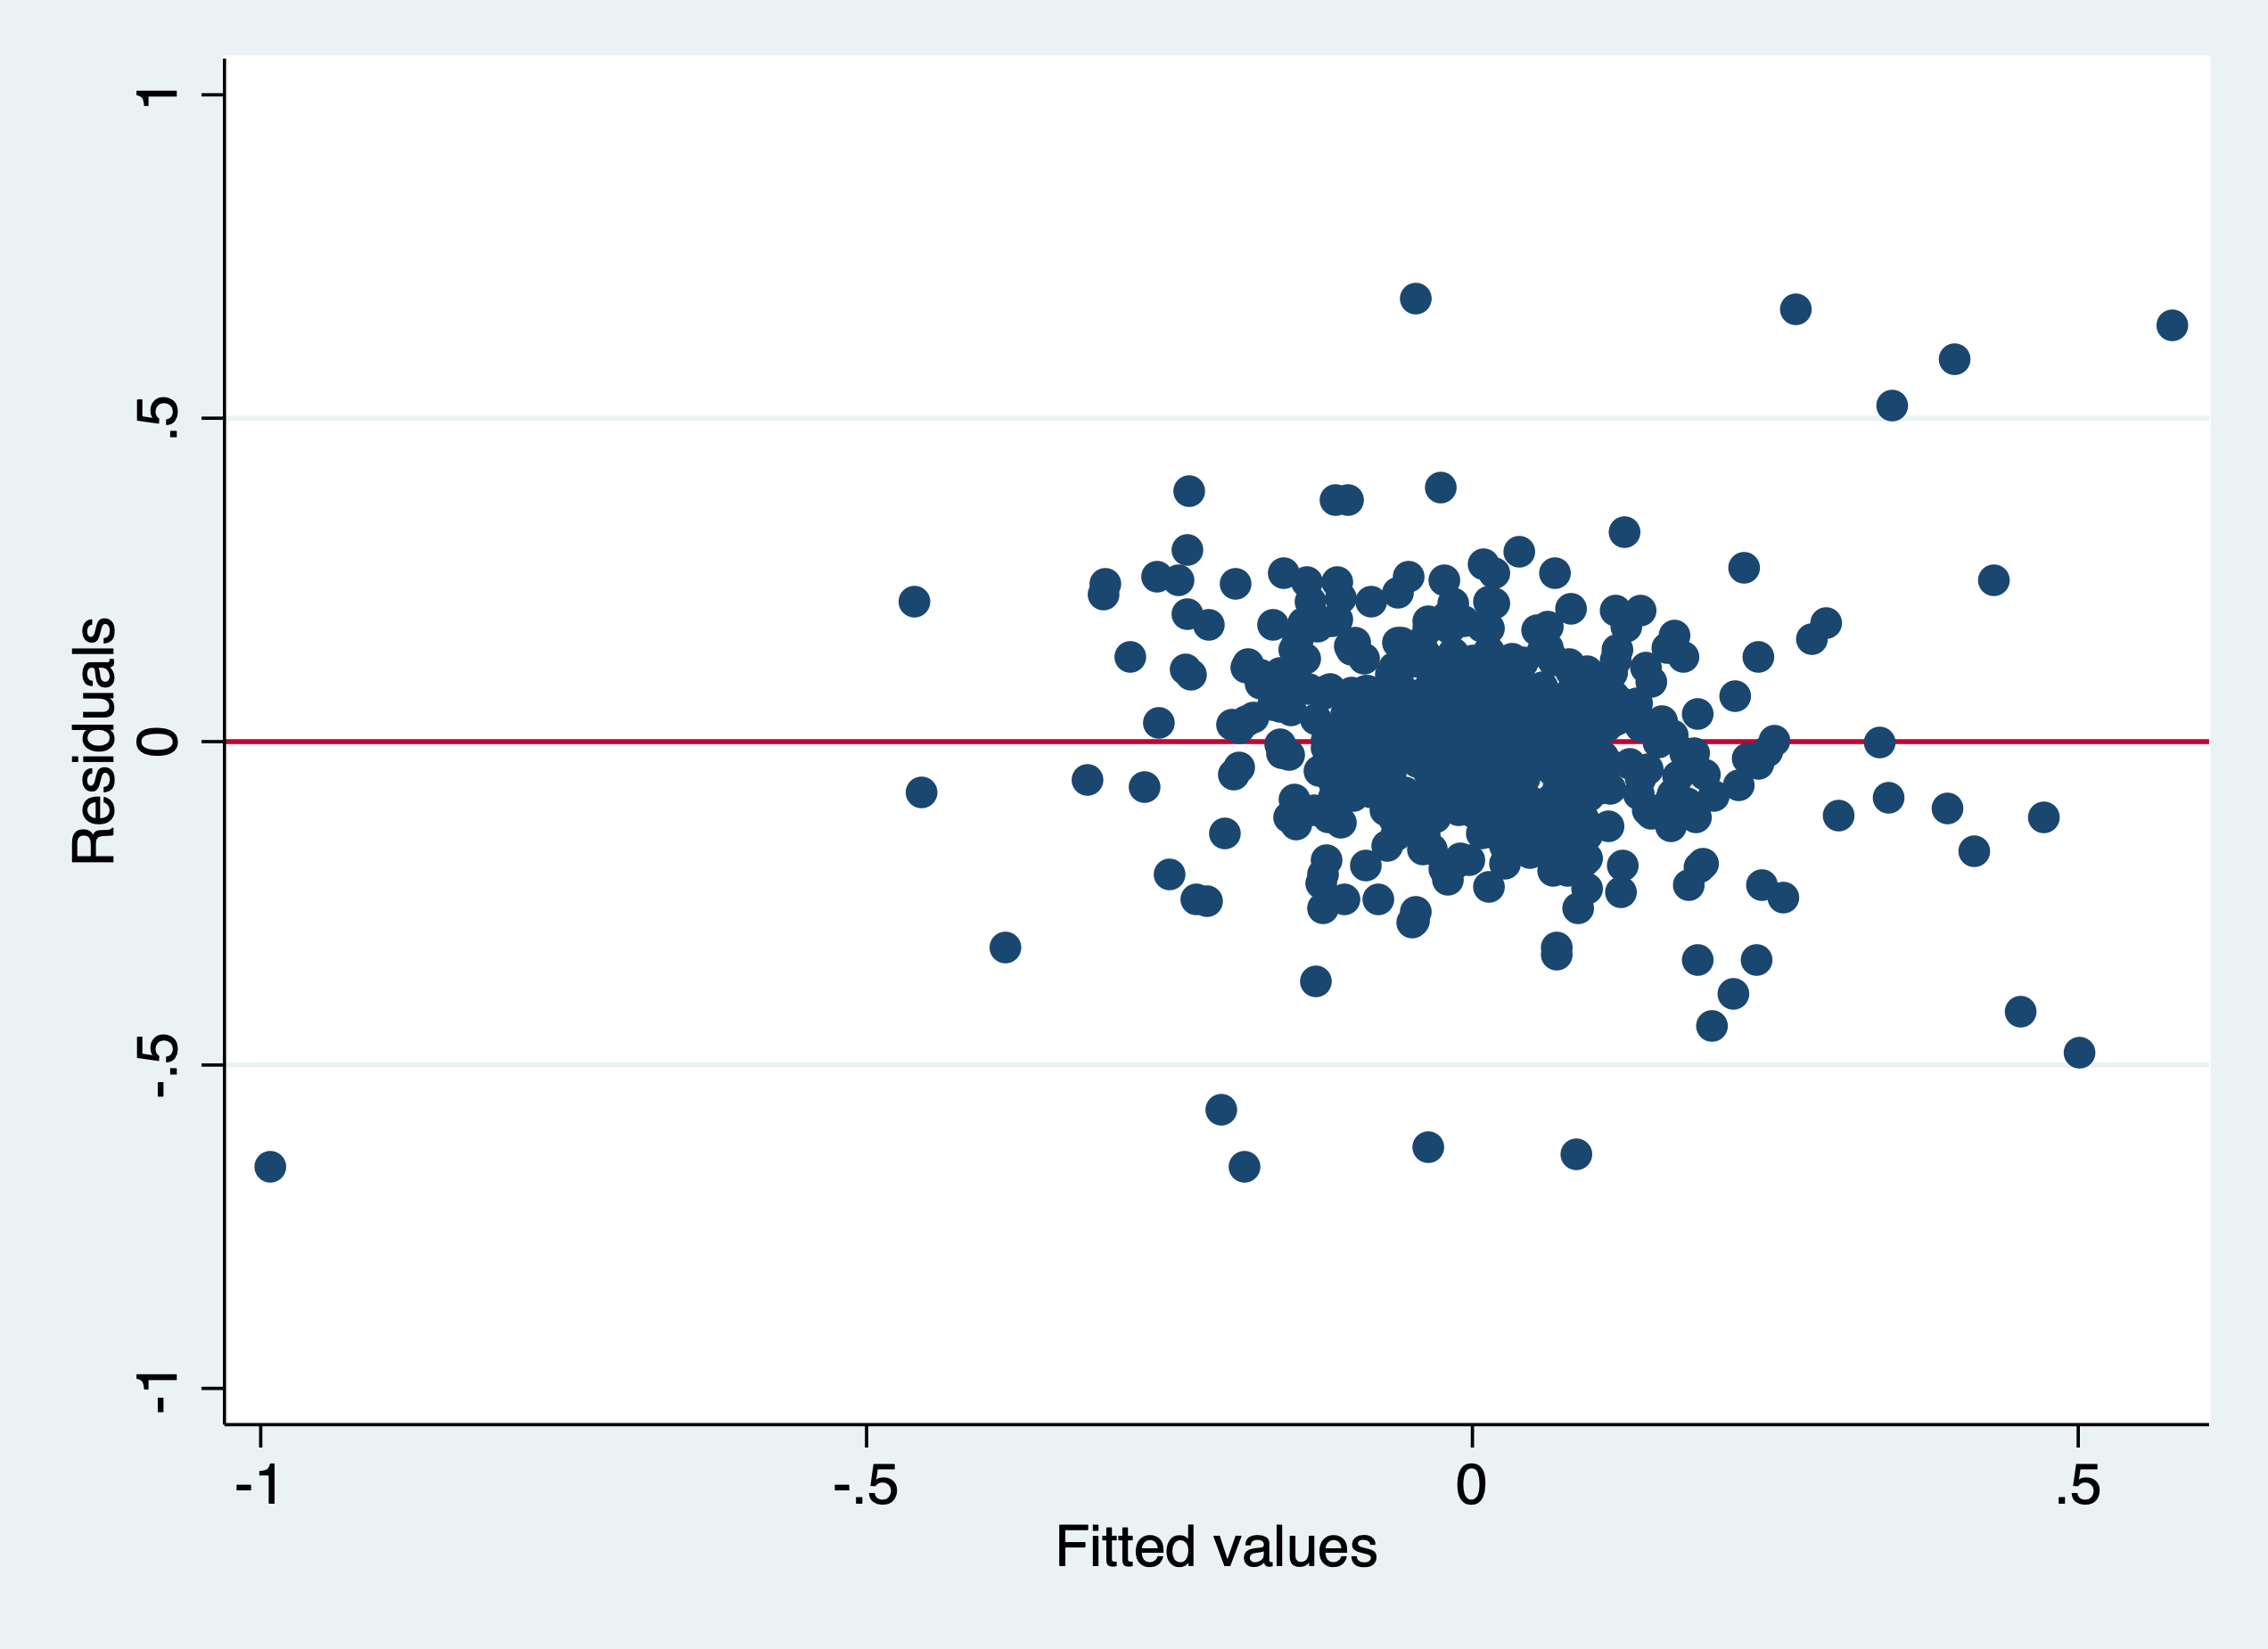
\includegraphics[keepaspectratio]{week3_htsk.png}}
\caption{Plotting Errors}
\end{figure}

We can use the White Test and Breusch-Pagan, which yield different results

\begin{Shaded}
\begin{Highlighting}[]
\KeywordTok{estat} \KeywordTok{imtest}\NormalTok{, }\BaseNTok{white}
\KeywordTok{estat} \KeywordTok{hettest}
\end{Highlighting}
\end{Shaded}

\begin{verbatim}
White's test for Ho: homoskedasticity
         against Ha: unrestricted heteroskedasticity

         chi2(50)     =    257.57
         Prob > chi2  =    0.0000

Cameron & Trivedi's decomposition of IM-test

---------------------------------------------------
              Source |       chi2     df      p
---------------------+-----------------------------
  Heteroskedasticity |     257.57     50    0.0000
            Skewness |      62.96     10    0.0000
            Kurtosis |      12.82      1    0.0003
---------------------+-----------------------------
               Total |     333.35     61    0.0000
---------------------------------------------------


Breusch-Pagan / Cook-Weisberg test for heteroskedasticity 
         Ho: Constant variance
         Variables: fitted values of D.lcrmrte

         chi2(1)      =     1.16
         Prob > chi2  =   0.2807
\end{verbatim}

Re-estimate with Robust Standard Errors clustered at the county level and cluster by county (deal with error correlations within counties).

\begin{Shaded}
\begin{Highlighting}[]
\KeywordTok{reg} \KeywordTok{d}\NormalTok{.lcrmrte i.d83 i.d84 i.d85 i.d86 i.d87 }\KeywordTok{d}\NormalTok{.lprbarr }\KeywordTok{d}\NormalTok{.lprbconv }\KeywordTok{d}\NormalTok{.lprbpris }\KeywordTok{d}\NormalTok{.lavgsen }\KeywordTok{d}\NormalTok{.lpolpc, }\KeywordTok{robust} \KeywordTok{cluster}\NormalTok{(county)}
\end{Highlighting}
\end{Shaded}

\begin{verbatim}
Linear regression                               Number of obs     =        540
                                                F(10, 89)         =      13.56
                                                Prob > F          =     0.0000
                                                R-squared         =     0.4325
                                                Root MSE          =     .15431

                                (Std. Err. adjusted for 90 clusters in county)
------------------------------------------------------------------------------
             |               Robust
   D.lcrmrte |      Coef.   Std. Err.      t    P>|t|     [95% Conf. Interval]
-------------+----------------------------------------------------------------
       1.d83 |  -.0998658   .0222563    -4.49   0.000    -.1440887    -.055643
       1.d84 |  -.0479374   .0200531    -2.39   0.019    -.0877825   -.0080923
       1.d85 |  -.0046111     .02503    -0.18   0.854    -.0543453     .045123
       1.d86 |   .0275143   .0211829     1.30   0.197    -.0145756    .0696043
       1.d87 |   .0408267   .0241102     1.69   0.094    -.0070797    .0887331
             |
     lprbarr |
         D1. |  -.3274942   .0564281    -5.80   0.000    -.4396157   -.2153727
             |
    lprbconv |
         D1. |  -.2381066   .0395843    -6.02   0.000    -.3167598   -.1594534
             |
    lprbpris |
         D1. |  -.1650462   .0457923    -3.60   0.001    -.2560345    -.074058
             |
     lavgsen |
         D1. |  -.0217607     .02582    -0.84   0.402    -.0730644     .029543
             |
      lpolpc |
         D1. |   .3984264   .1029342     3.87   0.000     .1938983    .6029545
             |
       _cons |   .0077134   .0137846     0.56   0.577    -.0196763     .035103
------------------------------------------------------------------------------
\end{verbatim}

Even accounting for heteroskedasticity and serial correlation, our model is likely biased by simultaneity bias.

\chapter{Labeling Data}\label{labeling-data}

Mitchell's 5th chapter has a bunch of useful information, but the most
important parts are \emph{label define} (and its two options of \emph{add} and \emph{modify}), \emph{label values}, and time formatting.

\section{Describing datasets}\label{describing-datasets}

We have seen the \emph{describe} command before, but it is a very useful command to being working with data. It provides the varible name, storage type, display format, value label, and variable label, Let's get some data on the survey of graduate students.

\begin{Shaded}
\begin{Highlighting}[]
\NormalTok{cd }\StringTok{"/Users/Sam/Desktop/Econ 645/Data/Mitchell"}
\KeywordTok{use} \StringTok{"survey7.dta"}\NormalTok{, }\KeywordTok{clear}
\KeywordTok{describe}
\end{Highlighting}
\end{Shaded}

\begin{verbatim}
/Users/Sam/Desktop/Econ 645/Data/Mitchell

(Survey of graduate students)


Contains data from survey7.dta
  obs:             8                          Survey of graduate students
 vars:            11                          5 May 2020 14:37
 size:           400                          (_dta has notes)
------------------------------------------------------------------------------------------------------------------
              storage   display    value
variable name   type    format     label      variable label
------------------------------------------------------------------------------------------------------------------
id              float   %9.0g                 Unique identification variable
STUDENTVARS     float   %9.0g                 STUDENT VARIABLES ===============
gender          float   %9.0g      mf         Gender of student
race            float   %19.0g     racelab  * Race of student
bday            float   %td..                 Date of birth of student
income          float   %11.1fc               Income of student
havechild       float   %18.0g     havelab  * Given birth to a child?
KIDVARS         float   %9.0g                 KID VARIABLES ===================
kidname         str10   %-10s                 Name of child
ksex            float   %15.0g     mfkid    * Sex of child
kbday           float   %td..                 Date of birth of child
                                            * indicated variables have notes
------------------------------------------------------------------------------------------------------------------
Sorted by: 
\end{verbatim}

We also have a short option, but it just contain general information.

\begin{Shaded}
\begin{Highlighting}[]
\KeywordTok{describe}\NormalTok{, }\KeywordTok{short}
\end{Highlighting}
\end{Shaded}

\begin{verbatim}
Contains data from survey7.dta
  obs:             8                          Survey of graduate students
 vars:            11                          5 May 2020 14:37
 size:           400                          
Sorted by: 
\end{verbatim}

We can subset the variables we want to describe if we want

\begin{Shaded}
\begin{Highlighting}[]
\KeywordTok{describe}\NormalTok{ id gender race}
\end{Highlighting}
\end{Shaded}

\begin{verbatim}
              storage   display    value
variable name   type    format     label      variable label
------------------------------------------------------------------------------------------------------------------
id              float   %9.0g                 Unique identification variable
gender          float   %9.0g      mf         Gender of student
race            float   %19.0g     racelab  * Race of student
\end{verbatim}

Finally, the command \emph{codebook} provides a deep dive into your dataset. This is very useful for looking at the value labels. We only see the value label name in the \emph{describe} command, but the \emph{codebook} command provides more information, such as type of variable, label name, range of values, unique values, missing, value labels, missing value labels (if any).

\begin{Shaded}
\begin{Highlighting}[]
\KeywordTok{codebook}
\end{Highlighting}
\end{Shaded}

\begin{verbatim}
id                                                                                  Unique identification variable
------------------------------------------------------------------------------------------------------------------

                  type:  numeric (float)

                 range:  [1,8]                        units:  1
         unique values:  8                        missing .:  0/8

            tabulation:  Freq.  Value
                             1  1
                             1  2
                             1  3
                             1  4
                             1  5
                             1  6
                             1  7
                             1  8

------------------------------------------------------------------------------------------------------------------
STUDENTVARS                                                                      STUDENT VARIABLES ===============
------------------------------------------------------------------------------------------------------------------

                  type:  numeric (float)

                 range:  [.,.]                        units:  .
         unique values:  0                        missing .:  8/8

            tabulation:  Freq.  Value
                             8  .

------------------------------------------------------------------------------------------------------------------
gender                                                                                           Gender of student
------------------------------------------------------------------------------------------------------------------

                  type:  numeric (float)
                 label:  mf

                 range:  [1,2]                        units:  1
         unique values:  2                        missing .:  0/8

            tabulation:  Freq.   Numeric  Label
                             3         1  Male
                             5         2  Female

------------------------------------------------------------------------------------------------------------------
race                                                                                               Race of student
------------------------------------------------------------------------------------------------------------------

                  type:  numeric (float)
                 label:  racelab

                 range:  [1,5]                        units:  1
         unique values:  5                        missing .:  0/8

            tabulation:  Freq.   Numeric  Label
                             2         1  White
                             2         2  Asian
                             2         3  Hispanic
                             1         4  African American
                             1         5  Other

------------------------------------------------------------------------------------------------------------------
bday                                                                                      Date of birth of student
------------------------------------------------------------------------------------------------------------------

                  type:  numeric daily date (float)

                 range:  [389,7935]                   units:  1
       or equivalently:  [24jan1961,22sep1981]        units:  days
         unique values:  8                        missing .:  0/8

            tabulation:  Freq.  Value
                             1  389    24jan1961
                             1  3027   15apr1968
                             1  4160   23may1971
                             1  4924   25jun1973
                             1  5036   15oct1973
                             1  6059   03aug1976
                             1  6391   01jul1977
                             1  7935   22sep1981

------------------------------------------------------------------------------------------------------------------
income                                                                                           Income of student
------------------------------------------------------------------------------------------------------------------

                  type:  numeric (float)

                 range:  [545.23,1284354.5]           units:  .01
         unique values:  8                        missing .:  0/8

            tabulation:  Freq.  Value
                             1  545.22998
                             1  4500.9199
                             1  10500.93
                             1  45234.129
                             1  109452.11
                             1  120102.32
                             1  124313.45
                             1  1284354.5

------------------------------------------------------------------------------------------------------------------
havechild                                                                                  Given birth to a child?
------------------------------------------------------------------------------------------------------------------

                  type:  numeric (float)
                 label:  havelab

                 range:  [0,1]                        units:  1
         unique values:  2                        missing .:  0/8
       unique mv codes:  1                       missing .*:  3/8

            tabulation:  Freq.   Numeric  Label
                             1         0  Dont Have Child
                             4         1  Have Child
                             3        .n  NA

------------------------------------------------------------------------------------------------------------------
KIDVARS                                                                          KID VARIABLES ===================
------------------------------------------------------------------------------------------------------------------

                  type:  numeric (float)

                 range:  [.,.]                        units:  .
         unique values:  0                        missing .:  8/8

            tabulation:  Freq.  Value
                             8  .

------------------------------------------------------------------------------------------------------------------
kidname                                                                                              Name of child
------------------------------------------------------------------------------------------------------------------

                  type:  string (str10), but longest is str9

         unique values:  5                        missing "":  0/8

            tabulation:  Freq.  Value
                             4  ""
                             1  "Catherine"
                             1  "Robin"
                             1  "Sally"
                             1  "Samuell"

               warning:  variable has leading and trailing blanks

------------------------------------------------------------------------------------------------------------------
ksex                                                                                                  Sex of child
------------------------------------------------------------------------------------------------------------------

                  type:  numeric (float)
                 label:  mfkid

                 range:  [1,2]                        units:  1
         unique values:  2                        missing .:  0/8
       unique mv codes:  2                       missing .*:  5/8

            tabulation:  Freq.   Numeric  Label
                             1         1  Male
                             2         2  Female
                             4        .n  NA
                             1        .u  Unknown

------------------------------------------------------------------------------------------------------------------
kbday                                                                                       Date of birth of child
------------------------------------------------------------------------------------------------------------------

                  type:  numeric daily date (float)

                 range:  [12888,15932]                units:  1
       or equivalently:  [15apr1995,15aug2003]        units:  days
         unique values:  4                        missing .:  4/8

            tabulation:  Freq.  Value
                             1  12888  15apr1995
                             1  14019  20may1998
                             1  14256  12jan1999
                             1  15932  15aug2003
                             4  .              .
\end{verbatim}

We can go by variables.

\begin{Shaded}
\begin{Highlighting}[]
\KeywordTok{codebook}\NormalTok{ race}
\end{Highlighting}
\end{Shaded}

\begin{verbatim}
race                                                                                               Race of student
------------------------------------------------------------------------------------------------------------------

                  type:  numeric (float)
                 label:  racelab

                 range:  [1,5]                        units:  1
         unique values:  5                        missing .:  0/8

            tabulation:  Freq.   Numeric  Label
                             2         1  White
                             2         2  Asian
                             2         3  Hispanic
                             1         4  African American
                             1         5  Other
\end{verbatim}

We can go by variables and notes

\begin{Shaded}
\begin{Highlighting}[]
\KeywordTok{codebook}\NormalTok{ havechild, }\KeywordTok{notes}
\end{Highlighting}
\end{Shaded}

\begin{verbatim}
havechild                                                                                  Given birth to a child?
------------------------------------------------------------------------------------------------------------------

                  type:  numeric (float)
                 label:  havelab

                 range:  [0,1]                        units:  1
         unique values:  2                        missing .:  0/8
       unique mv codes:  1                       missing .*:  3/8

            tabulation:  Freq.   Numeric  Label
                             1         0  Dont Have Child
                             4         1  Have Child
                             3        .n  NA

havechild:
  1.  This variable measures whether a woman has given birth to a child, not just whether she is a parent.
  2.  The .n (NA) missing code is used for males, because they cannot bear children.
  3.  The .u (Unknown) missing code for a female indicating it is unknown if she has a child.
\end{verbatim}

We can look at the variable and missing value labels with the option \emph{mv}. I recommend that you don't label the missing values unless it is absolutely necessary. Different types of missing values besides ``.'' cause problems down the road, especially with the \emph{marginsplot} command.

\begin{Shaded}
\begin{Highlighting}[]
\KeywordTok{codebook}\NormalTok{ ksex, mv}
\end{Highlighting}
\end{Shaded}

\begin{verbatim}
ksex                                                                                                  Sex of child
------------------------------------------------------------------------------------------------------------------

                  type:  numeric (float)
                 label:  mfkid

                 range:  [1,2]                        units:  1
         unique values:  2                        missing .:  0/8
       unique mv codes:  2                       missing .*:  5/8

            tabulation:  Freq.   Numeric  Label
                             1         1  Male
                             2         2  Female
                             4        .n  NA
                             1        .u  Unknown

        missing values:     havechild==mv --> ksex==mv
                                kbday==mv --> ksex==mv
\end{verbatim}

If you are interested in the different languages labels it is on page 112.

The \emph{lookfor} command will return all variables with the search word. This is a bit redundent, since this is available in the variable window. But, it provides more space to look.

\begin{Shaded}
\begin{Highlighting}[]
\KeywordTok{lookfor}\NormalTok{ birth}
\end{Highlighting}
\end{Shaded}

\begin{verbatim}
              storage   display    value
variable name   type    format     label      variable label
------------------------------------------------------------------------------------------------------------------
bday            float   %td..                 Date of birth of student
havechild       float   %18.0g     havelab  * Given birth to a child?
kbday           float   %td..                 Date of birth of child
\end{verbatim}

We can also search for the notes by the search word

\begin{Shaded}
\begin{Highlighting}[]
\KeywordTok{notes} \KeywordTok{search}\NormalTok{ birth}
\end{Highlighting}
\end{Shaded}

\begin{verbatim}
havechild:
  1.  This variable measures whether a woman has given birth to a child, not just whether she is a parent.
\end{verbatim}

We can see the formats of the variables as well

\begin{Shaded}
\begin{Highlighting}[]
\OtherTok{list}\NormalTok{ income bday}
\KeywordTok{describe}\NormalTok{ income bday}
\end{Highlighting}
\end{Shaded}

\begin{verbatim}
     |      income       bday |
     |------------------------|
  1. |    10,500.9   01/24/61 |
  2. |    45,234.1   04/15/68 |
  3. | 1,284,354.5   05/23/71 |
  4. |   124,313.5   06/25/73 |
  5. |   120,102.3   09/22/81 |
     |------------------------|
  6. |       545.2   10/15/73 |
  7. |   109,452.1   07/01/77 |
  8. |     4,500.9   08/03/76 |
     +------------------------+

              storage   display    value
variable name   type    format     label      variable label
------------------------------------------------------------------------------------------------------------------
income          float   %11.1fc               Income of student
bday            float   %td..                 Date of birth of student
\end{verbatim}

We can see that the format for income is \%11.1fc and the format for bday is \%td

\section{Labeling variables}\label{labeling-variables}

Labeling the variables is a very helpful shortcut to describe what the variable contain without having to go back to the data dicionary. Sometimes we want a short and concise label if we are exporting labels to regression tables, or sometimes we want longer variable labels to give us context of the variable.

Let's get some data on graduate students and use the \emph{describe} command.

\begin{Shaded}
\begin{Highlighting}[]
\NormalTok{cd }\StringTok{"/Users/Sam/Desktop/Econ 645/Data/Mitchell"}
\KeywordTok{use} \StringTok{"survey1.dta"}\NormalTok{, }\KeywordTok{clear}
\KeywordTok{describe} 
\end{Highlighting}
\end{Shaded}

\begin{verbatim}
/Users/Sam/Desktop/Econ 645/Data/Mitchell



Contains data from survey1.dta
  obs:             8                          
 vars:             9                          1 Jan 2010 12:13
 size:           432                          
------------------------------------------------------------------------------------------------------------------
              storage   display    value
variable name   type    format     label      variable label
------------------------------------------------------------------------------------------------------------------
id              float   %9.0g                 
gender          float   %9.0g                 
race            float   %9.0g                 
havechild       float   %9.0g                 
ksex            float   %9.0g                 
bdays           str10   %10s                  
income          float   %9.0g                 
kbdays          str10   %10s                  
kidname         str10   %10s                  
------------------------------------------------------------------------------------------------------------------
Sorted by: 
\end{verbatim}

We have no variable labels, so we will need to provide some so future users have an understand what the data are. We will use the \emph{label variable} command to describe the variable.

\begin{Shaded}
\begin{Highlighting}[]
\KeywordTok{label} \KeywordTok{variable}\NormalTok{ id }\StringTok{"Identification variable"}
\KeywordTok{label} \KeywordTok{variable}\NormalTok{ gender }\StringTok{"Gender of the student"}
\KeywordTok{label} \KeywordTok{variable}\NormalTok{ race }\StringTok{"Race of the student"}
\KeywordTok{label} \KeywordTok{variable}\NormalTok{ havechild }\StringTok{"Given birth to a child"}
\KeywordTok{label} \KeywordTok{variable}\NormalTok{ ksex }\StringTok{"Sex of child"}
\KeywordTok{label} \KeywordTok{variable}\NormalTok{ bday }\StringTok{"Birthday of student"}
\KeywordTok{label} \KeywordTok{variable}\NormalTok{ income }\StringTok{"Income of student"}
\KeywordTok{label} \KeywordTok{variable}\NormalTok{ kbdays }\StringTok{"Birthday of child"}
\KeywordTok{label} \KeywordTok{variable}\NormalTok{ kidname }\StringTok{"Name of child"}
\KeywordTok{describe}
\end{Highlighting}
\end{Shaded}

\begin{verbatim}
Contains data from survey1.dta
  obs:             8                          
 vars:             9                          1 Jan 2010 12:13
 size:           432                          
------------------------------------------------------------------------------------------------------------------
              storage   display    value
variable name   type    format     label      variable label
------------------------------------------------------------------------------------------------------------------
id              float   %9.0g                 Identification variable
gender          float   %9.0g                 Gender of the student
race            float   %9.0g                 Race of the student
havechild       float   %9.0g                 Given birth to a child
ksex            float   %9.0g                 Sex of child
bdays           str10   %10s                  Birthday of student
income          float   %9.0g                 Income of student
kbdays          str10   %10s                  Birthday of child
kidname         str10   %10s                  Name of child
------------------------------------------------------------------------------------------------------------------
Sorted by: 
\end{verbatim}

We can simply change the variable label with running the command again with the new variable label.

\begin{Shaded}
\begin{Highlighting}[]
\KeywordTok{label} \KeywordTok{variable}\NormalTok{ id }\StringTok{"Unique identification variable"}
\KeywordTok{describe}
\KeywordTok{save}\NormalTok{ survey2, }\KeywordTok{replace}
\end{Highlighting}
\end{Shaded}

\begin{verbatim}
Contains data from survey1.dta
  obs:             8                          
 vars:             9                          1 Jan 2010 12:13
 size:           432                          
------------------------------------------------------------------------------------------------------------------
              storage   display    value
variable name   type    format     label      variable label
------------------------------------------------------------------------------------------------------------------
id              float   %9.0g                 Unique identification variable
gender          float   %9.0g                 Gender of the student
race            float   %9.0g                 Race of the student
havechild       float   %9.0g                 Given birth to a child
ksex            float   %9.0g                 Sex of child
bdays           str10   %10s                  Birthday of student
income          float   %9.0g                 Income of student
kbdays          str10   %10s                  Birthday of child
kidname         str10   %10s                  Name of child
------------------------------------------------------------------------------------------------------------------
Sorted by: 

file survey2.dta saved
\end{verbatim}

\section{Labeling values}\label{labeling-values}

Labeling values is a very practice way of analyzing data without having to go back to the data dictionary. Labeling values requires two commands:

\begin{enumerate}
\def\labelenumi{\arabic{enumi}.}
\tightlist
\item
  \emph{label define} to define a label that can be used across many different variables.
\item
  \emph{label variable} to place a label onto a variable.
\end{enumerate}

Labeling values is a bit different than labeling variables, since we need to modify or replace after a label has been defined. If you try to change a label, then you will get an error unless you use \emph{add}, \emph{modify} or \emph{replace}

Let's look at our codebook

\begin{Shaded}
\begin{Highlighting}[]
\NormalTok{cd }\StringTok{"/Users/Sam/Desktop/Econ 645/Data/Mitchell"}
\KeywordTok{use}\NormalTok{ survey2, }\KeywordTok{clear}
\KeywordTok{codebook} 
\end{Highlighting}
\end{Shaded}

\begin{verbatim}
/Users/Sam/Desktop/Econ 645/Data/Mitchell



------------------------------------------------------------------------------------------------------------------
id                                                                                  Unique identification variable
------------------------------------------------------------------------------------------------------------------

                  type:  numeric (float)

                 range:  [1,8]                        units:  1
         unique values:  8                        missing .:  0/8

            tabulation:  Freq.  Value
                             1  1
                             1  2
                             1  3
                             1  4
                             1  5
                             1  6
                             1  7
                             1  8

------------------------------------------------------------------------------------------------------------------
gender                                                                                       Gender of the student
------------------------------------------------------------------------------------------------------------------

                  type:  numeric (float)

                 range:  [1,2]                        units:  1
         unique values:  2                        missing .:  0/8

            tabulation:  Freq.  Value
                             3  1
                             5  2

------------------------------------------------------------------------------------------------------------------
race                                                                                           Race of the student
------------------------------------------------------------------------------------------------------------------

                  type:  numeric (float)

                 range:  [1,5]                        units:  1
         unique values:  5                        missing .:  0/8

            tabulation:  Freq.  Value
                             2  1
                             2  2
                             2  3
                             1  4
                             1  5

------------------------------------------------------------------------------------------------------------------
havechild                                                                                   Given birth to a child
------------------------------------------------------------------------------------------------------------------

                  type:  numeric (float)

                 range:  [0,1]                        units:  1
         unique values:  2                        missing .:  0/8
       unique mv codes:  1                       missing .*:  3/8

            tabulation:  Freq.  Value
                             1  0
                             4  1
                             3  .n

------------------------------------------------------------------------------------------------------------------
ksex                                                                                                  Sex of child
------------------------------------------------------------------------------------------------------------------

                  type:  numeric (float)

                 range:  [1,2]                        units:  1
         unique values:  2                        missing .:  0/8
       unique mv codes:  2                       missing .*:  5/8

            tabulation:  Freq.  Value
                             1  1
                             2  2
                             4  .n
                             1  .u

------------------------------------------------------------------------------------------------------------------
bdays                                                                                          Birthday of student
------------------------------------------------------------------------------------------------------------------

                  type:  string (str10)

         unique values:  8                        missing "":  0/8

            tabulation:  Freq.  Value
                             1  "1/24/1961"
                             1  "10/15/1973"
                             1  "4/15/1968"
                             1  "5/23/1971"
                             1  "6/25/1973"
                             1  "7/1/1977"
                             1  "8/3/1976"
                             1  "9/22/1981"

------------------------------------------------------------------------------------------------------------------
income                                                                                           Income of student
------------------------------------------------------------------------------------------------------------------

                  type:  numeric (float)

                 range:  [545.23,1284354.5]           units:  .01
         unique values:  8                        missing .:  0/8

            tabulation:  Freq.  Value
                             1  545.22998
                             1  4500.9199
                             1  10500.93
                             1  45234.129
                             1  109452.11
                             1  120102.32
                             1  124313.45
                             1  1284354.5

------------------------------------------------------------------------------------------------------------------
kbdays                                                                                           Birthday of child
------------------------------------------------------------------------------------------------------------------

                  type:  string (str10), but longest is str9

         unique values:  5                        missing "":  0/8

            tabulation:  Freq.  Value
                             4  ""
                             1  "1/12/1999"
                             1  "4/15/1995"
                             1  "5/20/1998"
                             1  "8/15/2003"

               warning:  variable has leading and trailing blanks

------------------------------------------------------------------------------------------------------------------
kidname                                                                                              Name of child
------------------------------------------------------------------------------------------------------------------

                  type:  string (str10), but longest is str9

         unique values:  5                        missing "":  0/8

            tabulation:  Freq.  Value
                             4  ""
                             1  "Catherine"
                             1  "Robin"
                             1  "Sally"
                             1  "Samuell"

               warning:  variable has leading and trailing blanks
\end{verbatim}

We have our variable labels from 5.3, but now we need to label the values so replicators can know what the data are without having to reference the data dictionary for every variable. We will use the \emph{label define} command to create a new label.

First we need to define a label with label define

\begin{Shaded}
\begin{Highlighting}[]
\KeywordTok{label} \KeywordTok{define}\NormalTok{ racelabel 1 }\StringTok{"White"}\NormalTok{ 2 }\StringTok{"Asian"}\NormalTok{ 3 }\StringTok{"Hispanic"}\NormalTok{ 4 }\StringTok{"Black"}
\end{Highlighting}
\end{Shaded}

Next we need to label the values of the variable with \emph{label values} command and we'll look at the codebook again.

\begin{Shaded}
\begin{Highlighting}[]
\KeywordTok{label} \KeywordTok{values}\NormalTok{ race racelabel}
\KeywordTok{codebook}\NormalTok{ race}
\end{Highlighting}
\end{Shaded}

\begin{verbatim}
race                                                                                           Race of the student
------------------------------------------------------------------------------------------------------------------

                  type:  numeric (float)
                 label:  racelabel, but 1 nonmissing value is not labeled

                 range:  [1,5]                        units:  1
         unique values:  5                        missing .:  0/8

            tabulation:  Freq.   Numeric  Label
                             2         1  White
                             2         2  Asian
                             2         3  Hispanic
                             1         4  Black
                             1         5  
\end{verbatim}

We are still missing a value label for 5, which is Other, so we need to modify our defined label race1. If we do not modify our label, we will get an error if we try to label values again. We can use the \emph{add} option in label define.

\begin{Shaded}
\begin{Highlighting}[]
\KeywordTok{label} \KeywordTok{define}\NormalTok{ racelabel 5 }\StringTok{"Other"}\NormalTok{, add}
\end{Highlighting}
\end{Shaded}

If we want to modify an existing label, we can use the \emph{modify} option in label define.

\begin{Shaded}
\begin{Highlighting}[]
\KeywordTok{label} \KeywordTok{define}\NormalTok{ racelabel 4 }\StringTok{"African American"}\NormalTok{, modify}
\KeywordTok{codebook}\NormalTok{ race}
\end{Highlighting}
\end{Shaded}

\begin{verbatim}
race                                                                                           Race of the student
------------------------------------------------------------------------------------------------------------------

                  type:  numeric (float)
                 label:  racelabel

                 range:  [1,5]                        units:  1
         unique values:  5                        missing .:  0/8

            tabulation:  Freq.   Numeric  Label
                             2         1  White
                             2         2  Asian
                             2         3  Hispanic
                             1         4  African American
                             1         5  Other
\end{verbatim}

Labeling missing is something that I don't recommend, but we'll show an example here.

\begin{Shaded}
\begin{Highlighting}[]
\KeywordTok{label} \KeywordTok{define}\NormalTok{ mfkid 1 }\StringTok{"Male"}\NormalTok{ 2 }\StringTok{"Female"}\NormalTok{ .u }\StringTok{"Unknown"}\NormalTok{ .n }\StringTok{"NA"}
\KeywordTok{label} \KeywordTok{values}\NormalTok{ ksex mfkid}
\KeywordTok{codebook}\NormalTok{ ksex}

\KeywordTok{label} \KeywordTok{define}\NormalTok{ havechildlabel 0 }\StringTok{"Don\textquotesingle{}t have a child"}\NormalTok{ 1 }\StringTok{"Have a child"}\NormalTok{ .u }\StringTok{"Unknown"}\NormalTok{ .n }\StringTok{"NA"}
\KeywordTok{label} \KeywordTok{values}\NormalTok{ havechild havechildlabel}
\KeywordTok{codebook}\NormalTok{ havechild}
\end{Highlighting}
\end{Shaded}

\begin{verbatim}
ksex                                                                                                  Sex of child
------------------------------------------------------------------------------------------------------------------

                  type:  numeric (float)
                 label:  mfkid

                 range:  [1,2]                        units:  1
         unique values:  2                        missing .:  0/8
       unique mv codes:  2                       missing .*:  5/8

            tabulation:  Freq.   Numeric  Label
                             1         1  Male
                             2         2  Female
                             4        .n  NA
                             1        .u  Unknown




------------------------------------------------------------------------------------------------------------------
havechild                                                                                   Given birth to a child
------------------------------------------------------------------------------------------------------------------

                  type:  numeric (float)
                 label:  havechildlabel

                 range:  [0,1]                        units:  1
         unique values:  2                        missing .:  0/8
       unique mv codes:  1                       missing .*:  3/8

            tabulation:  Freq.   Numeric  Label
                             1         0  Don't have a child
                             4         1  Have a child
                             3        .n  NA
\end{verbatim}

We can look at our label list to see what we have define so far. We can use the \emph{label list} command to see our labels.

\begin{Shaded}
\begin{Highlighting}[]
\KeywordTok{label} \OtherTok{list}
\end{Highlighting}
\end{Shaded}

\begin{verbatim}
havechildlabel:
           0 Don't have a child
           1 Have a child
          .n NA
          .u Unknown
mfkid:
           1 Male
           2 Female
          .n NA
          .u Unknown
racelabel:
           1 White
           2 Asian
           3 Hispanic
           4 African American
           5 Other
\end{verbatim}

The \emph{numlabel} command is an interesting command. It takes the guess work out of knowing the numeric value of the category by appending the numeric value with the label value.

\begin{Shaded}
\begin{Highlighting}[]
\KeywordTok{numlabel}\NormalTok{ racelabel, add}
\KeywordTok{label} \OtherTok{list}\NormalTok{ racelabel}
\KeywordTok{tabulate}\NormalTok{ race}
\end{Highlighting}
\end{Shaded}

\begin{verbatim}
racelabel:
           1 1. White
           2 2. Asian
           3 3. Hispanic
           4 4. African American
           5 5. Other


Race of the |
    student |      Freq.     Percent        Cum.
------------+-----------------------------------
          1 |          2       25.00       25.00
          2 |          2       25.00       50.00
          3 |          2       25.00       75.00
          4 |          1       12.50       87.50
          5 |          1       12.50      100.00
------------+-----------------------------------
      Total |          8      100.00
\end{verbatim}

And, if we don't like it or don't need it any more, we can remove the numeric values with the \emph{remove} option.

\begin{Shaded}
\begin{Highlighting}[]
\KeywordTok{numlabel}\NormalTok{ racelabel, remove}
\KeywordTok{tabulate}\NormalTok{ race}
\end{Highlighting}
\end{Shaded}

\begin{verbatim}
Race of the |
    student |      Freq.     Percent        Cum.
------------+-----------------------------------
          1 |          2       25.00       25.00
          2 |          2       25.00       50.00
          3 |          2       25.00       75.00
          4 |          1       12.50       87.50
          5 |          1       12.50      100.00
------------+-----------------------------------
      Total |          8      100.00
\end{verbatim}

We can add additional characters with \emph{numlabel} as well, such as ``\#='' or ``\#)'' with the \emph{mask} option

\begin{Shaded}
\begin{Highlighting}[]
\KeywordTok{numlabel}\NormalTok{ racelabel, add mask(}\StringTok{"\#) "}\NormalTok{)}
\KeywordTok{tabulate}\NormalTok{ race}
\end{Highlighting}
\end{Shaded}

\begin{verbatim}
Race of the |
    student |      Freq.     Percent        Cum.
------------+-----------------------------------
          1 |          2       25.00       25.00
          2 |          2       25.00       50.00
          3 |          2       25.00       75.00
          4 |          1       12.50       87.50
          5 |          1       12.50      100.00
------------+-----------------------------------
      Total |          8      100.00
\end{verbatim}

We can remove the mask with \emph{remove} plus the \emph{mask} option

\begin{Shaded}
\begin{Highlighting}[]
\KeywordTok{numlabel}\NormalTok{ racelabel, remove mask(}\StringTok{"\#) "}\NormalTok{)}
\KeywordTok{tabulate}\NormalTok{ race}
\end{Highlighting}
\end{Shaded}

\begin{verbatim}
Race of the |
    student |      Freq.     Percent        Cum.
------------+-----------------------------------
          1 |          2       25.00       25.00
          2 |          2       25.00       50.00
          3 |          2       25.00       75.00
          4 |          1       12.50       87.50
          5 |          1       12.50      100.00
------------+-----------------------------------
      Total |          8      100.00
\end{verbatim}

\begin{Shaded}
\begin{Highlighting}[]
\KeywordTok{save}\NormalTok{ survey3, }\KeywordTok{replace}
\end{Highlighting}
\end{Shaded}

\section{Labeling utilities}\label{labeling-utilities}

Stata has label utilities to manage the labels defined. The first one is \emph{label dir} to see the labels names available in a quick and more concise way than using the codebook command.

For me, I think that \emph{label list} will be your most useful command here.

Quick check of your label directory

\begin{Shaded}
\begin{Highlighting}[]
\NormalTok{cd }\StringTok{"/Users/Sam/Desktop/Econ 645/Data/Mitchell"}
\KeywordTok{use}\NormalTok{ survey3, }\KeywordTok{clear}
\KeywordTok{label} \OtherTok{dir}
\end{Highlighting}
\end{Shaded}

\begin{verbatim}
/Users/Sam/Desktop/Econ 645/Data/Mitchell


mfkid
havechildlabel
racelabel
\end{verbatim}

The \emph{label list} command gives a more comprehensive view of your labels that includes the value labels associated with the value label name

\begin{Shaded}
\begin{Highlighting}[]
\KeywordTok{label} \OtherTok{list}
\end{Highlighting}
\end{Shaded}

\begin{verbatim}
mfkid:
           1 Male
           2 Female
          .n NA
          .u Unknown
havechildlabel:
           0 Don't have a child
           1 Have a child
          .n NA
          .u Unknown
racelabel:
           1 White
           2 Asian
           3 Hispanic
           4 African American
           5 Other
\end{verbatim}

The \emph{label save} command will save your labels into a do file for future use. Our do file name is stated after the using statement.

\begin{Shaded}
\begin{Highlighting}[]
\KeywordTok{label} \KeywordTok{save}\NormalTok{ havechildlabel racelabel }\KeywordTok{using}\NormalTok{ surveylabs, }\KeywordTok{replace}
\DecValTok{type}\NormalTok{ surveylabs.}\KeywordTok{do}
\end{Highlighting}
\end{Shaded}

\begin{verbatim}
label define havechildlabel 0 `"Don't have a child"', modify
label define havechildlabel 1 `"Have a child"', modify
label define havechildlabel .n `"NA"', modify
label define havechildlabel .u `"Unknown"', modify
label define racelabel 1 `"White"', modify
label define racelabel 2 `"Asian"', modify
label define racelabel 3 `"Hispanic"', modify
label define racelabel 4 `"African American"', modify
label define racelabel 5 `"Other"', modify
\end{verbatim}

The \emph{labelbook} command provides information similar to \emph{codebook} but only for the labels that are defined.

\begin{Shaded}
\begin{Highlighting}[]
\KeywordTok{labelbook}
\KeywordTok{labelbook}\NormalTok{ racelabel}
\end{Highlighting}
\end{Shaded}

\begin{verbatim}
value label havechildlabel 
------------------------------------------------------------------------------------------------------------------

      values                                    labels
       range:  [0,1]                     string length:  [2,18]
           N:  4                 unique at full length:  yes
        gaps:  no                  unique at length 12:  yes
  missing .*:  2                           null string:  no
                               leading/trailing blanks:  no
                                    numeric -> numeric:  no
  definition
           0   Don't have a child
           1   Have a child
          .n   NA
          .u   Unknown

   variables:  havechild


------------------------------------------------------------------------------------------------------------------
value label mfkid 
------------------------------------------------------------------------------------------------------------------

      values                                    labels
       range:  [1,2]                     string length:  [2,7]
           N:  4                 unique at full length:  yes
        gaps:  no                  unique at length 12:  yes
  missing .*:  2                           null string:  no
                               leading/trailing blanks:  no
                                    numeric -> numeric:  no
  definition
           1   Male
           2   Female
          .n   NA
          .u   Unknown

   variables:  ksex


------------------------------------------------------------------------------------------------------------------
value label racelabel 
------------------------------------------------------------------------------------------------------------------

      values                                    labels
       range:  [1,5]                     string length:  [5,16]
           N:  5                 unique at full length:  yes
        gaps:  no                  unique at length 12:  yes
  missing .*:  0                           null string:  no
                               leading/trailing blanks:  no
                                    numeric -> numeric:  no
  definition
           1   White
           2   Asian
           3   Hispanic
           4   African American
           5   Other

   variables:  race



------------------------------------------------------------------------------------------------------------------
value label racelabel 
------------------------------------------------------------------------------------------------------------------

      values                                    labels
       range:  [1,5]                     string length:  [5,16]
           N:  5                 unique at full length:  yes
        gaps:  no                  unique at length 12:  yes
  missing .*:  0                           null string:  no
                               leading/trailing blanks:  no
                                    numeric -> numeric:  no
  definition
           1   White
           2   Asian
           3   Hispanic
           4   African American
           5   Other

   variables:  race
\end{verbatim}

The \emph{problem} option for \emph{labelbook} provides information to alert the users of any problems

\begin{Shaded}
\begin{Highlighting}[]
\KeywordTok{labelbook}\NormalTok{, problem}
\end{Highlighting}
\end{Shaded}

\begin{verbatim}
no potential problems in dataset survey3.dta
\end{verbatim}

We can have a more detailed look with the \emph{detail} and \emph{problem} options

\begin{Shaded}
\begin{Highlighting}[]
\KeywordTok{labelbook}\NormalTok{ racelabel, problem }\KeywordTok{detail}
\end{Highlighting}
\end{Shaded}

\begin{verbatim}
value label racelabel 
------------------------------------------------------------------------------------------------------------------

      values                                    labels
       range:  [1,5]                     string length:  [5,16]
           N:  5                 unique at full length:  yes
        gaps:  no                  unique at length 12:  yes
  missing .*:  0                           null string:  no
                               leading/trailing blanks:  no
                                    numeric -> numeric:  no
  definition
           1   White
           2   Asian
           3   Hispanic
           4   African American
           5   Other

   variables:  race


no potential problems in dataset survey3.dta
\end{verbatim}

\section{Labeling variables and values in different languages}\label{labeling-variables-and-values-in-different-languages}

We will not be covering this, but if you are interested, please review pages 127-132.

\section{Using Notes}\label{using-notes}

The \emph{note} commmand can be helpful for future users or for replicators. If you use the \emph{note} command without specifying the variable, then it is a general note that will show up under the \_dta note. If you add a variable in front of the \emph{note} command, like note var1:, then you will add a note to the variable

Let's add some general notes.

\begin{Shaded}
\begin{Highlighting}[]
\KeywordTok{note}\NormalTok{: This was based }\KeywordTok{on}\NormalTok{ the dataset called survey1.txt}
\end{Highlighting}
\end{Shaded}

Adding \emph{TS} to the end adds a timestamp, which is a nice feature.

\begin{Shaded}
\begin{Highlighting}[]
\KeywordTok{note}\NormalTok{: The }\FunctionTok{missing} \KeywordTok{values} \KeywordTok{for}\NormalTok{ havechild and childage were coded }\KeywordTok{using}\NormalTok{ {-}1 and {-}2 but were converted to .n and .u TS}
\end{Highlighting}
\end{Shaded}

Let's call our notes with the \emph{notes} command.

\begin{Shaded}
\begin{Highlighting}[]
\KeywordTok{notes}
\end{Highlighting}
\end{Shaded}

\begin{verbatim}
_dta:
  1.  This was based on the dataset called survey1.txt
  2.  The missing values for havechild and childage were coded using -1 and -2 but were converted to .n and .u 27
      Aug 2025 16:45
\end{verbatim}

Let's add some notes to our variables

\begin{Shaded}
\begin{Highlighting}[]
\KeywordTok{note}\NormalTok{ race: The other category includes people who specified multiple races}
\KeywordTok{note}\NormalTok{ race: This is another }\KeywordTok{note}
\KeywordTok{note}\NormalTok{ race: This is a third }\KeywordTok{note}
\end{Highlighting}
\end{Shaded}

We can just call a particular variable for notes

\begin{Shaded}
\begin{Highlighting}[]
\KeywordTok{notes}\NormalTok{ race}
\end{Highlighting}
\end{Shaded}

We can just call a particular variable for notes

\begin{verbatim}
race:
  1.  The other category includes people who specified multiple races
  2.  This is another note
  3.  This is a third note
\end{verbatim}

Let say we added an unhelpful note, then we can drop it with the \emph{notes drop} command and we want to drop the second note.

\begin{Shaded}
\begin{Highlighting}[]
\KeywordTok{notes} \KeywordTok{drop}\NormalTok{ race }\KeywordTok{in}\NormalTok{ 2}
\KeywordTok{notes}\NormalTok{ race}
\end{Highlighting}
\end{Shaded}

\begin{verbatim}
  (1 note dropped)


race:
  1.  The other category includes people who specified multiple races
  3.  This is a third note
\end{verbatim}

Notice that we have a gap in the sequence of numbering. We can fix that with the \emph{notes renumber} command.

\begin{Shaded}
\begin{Highlighting}[]
\KeywordTok{notes}\NormalTok{ renumber race}
\KeywordTok{notes}\NormalTok{ race}
\end{Highlighting}
\end{Shaded}

\begin{verbatim}
race:
  1.  The other category includes people who specified multiple races
  2.  This is a third note
\end{verbatim}

We can also search notes with the notes search ``string'' command.

\begin{Shaded}
\begin{Highlighting}[]
\KeywordTok{notes} \KeywordTok{search}\NormalTok{ .u}
\end{Highlighting}
\end{Shaded}

\begin{verbatim}
_dta:
  2.  The missing values for havechild and childage were coded using -1 and -2 but were converted to .n and .u 27
      Aug 2025 16:45
\end{verbatim}

\section{Formatting the display of variables}\label{formatting-the-display-of-variables}

Formatting data will be more common than you expect. It can be a pain when dealing with numbers in the millions or billions and you lack commas. We can format our data with the \emph{format} command.

\subsection{Format numerics}\label{format-numerics}

Let's get our survey data and list the first 5 observations for id and income

Let's look at the format of income.

\begin{Shaded}
\begin{Highlighting}[]
\NormalTok{cd }\StringTok{"/Users/Sam/Desktop/Econ 645/Data/Mitchell"}
\KeywordTok{use}\NormalTok{ survey5, }\KeywordTok{clear}
\KeywordTok{describe}\NormalTok{ income}
\OtherTok{list}\NormalTok{ id income }\KeywordTok{in}\NormalTok{ 1/5}
\end{Highlighting}
\end{Shaded}

\begin{verbatim}
/Users/Sam/Desktop/Econ 645/Data/Mitchell

(Survey of graduate students)

              storage   display    value
variable name   type    format     label      variable label
------------------------------------------------------------------------------------------------------------------
income          float   %9.0g                 Income of student

     +---------------+
     | id     income |
     |---------------|
  1. |  1   10500.93 |
  2. |  2   45234.13 |
  3. |  3    1284355 |
  4. |  4   124313.5 |
  5. |  5   120102.3 |
     +---------------+
\end{verbatim}

The format is \emph{\%9.0g}. We always have \emph{\%} in front of our format and \emph{g} is a general way of displaying incomes using a width of nine digits and decides for us the best way to display the values. \emph{g} means general here.

\emph{\%.0g} means general - find the best way to show the decimals.

Note: \emph{\%.g} will change the format to exponent if necessary. Also \emph{} is usually set to 0 with \emph{g}.

\emph{\%.f} means fixed - \emph{w} is the width, \emph{d} is the decimals, and \emph{f} means fixed

\emph{\%.fc} means fixed with commas - \emph{w} is the width, \emph{d} is the decimals, \emph{f} means fixed, and \emph{c} means comma

\emph{\%.0gc} means general with commas - \emph{w} is the width, setting 0 means Stata will decide the decimals, \emph{g} means general, and \emph{c} means comma

The manual is helpful for formatting: \url{https://www.stata.com/manuals/dformat.pdf}

Example 1: \emph{format} v1 \emph{\%10.0g} - Width of 10 digits and decimals will be decided.

Example 2: \emph{format} v2 \emph{\%4.1f} - Show 3 digits in v3 and 1 decimal

Example 3: \emph{format} v3 \emph{\%6.1fc} - Show 4 digits plus the comma plus 1 digit

Let's get more control over the income format and use the \emph{\%w.df} format. We want a total of 12 digits with 2 decimals places, which means we have 10 digits on the left side of the ``.''

\begin{Shaded}
\begin{Highlighting}[]
\KeywordTok{format}\NormalTok{ income \%12.2f}
\OtherTok{list}\NormalTok{ income }\KeywordTok{in}\NormalTok{ 1/5}
\end{Highlighting}
\end{Shaded}

\begin{verbatim}
     |     income |
     |------------|
  1. |   10500.93 |
  2. |   45234.13 |
  3. | 1284354.50 |
  4. |  124313.45 |
  5. |  120102.32 |
     +------------+
\end{verbatim}

Notice that we now can see observation \#3's decimal places.

If we don't care to see the decimal place (even though it is still there).

\begin{Shaded}
\begin{Highlighting}[]
\KeywordTok{format}\NormalTok{ income \%7.0f}
\OtherTok{list}\NormalTok{ income }\KeywordTok{in}\NormalTok{ 1/5}
\end{Highlighting}
\end{Shaded}

\begin{verbatim}
     |  income |
     |---------|
  1. |   10501 |
  2. |   45234 |
  3. | 1284354 |
  4. |  124313 |
  5. |  120102 |
     +---------+
\end{verbatim}

We we want to see one decimal place

\begin{Shaded}
\begin{Highlighting}[]
\KeywordTok{format}\NormalTok{ income \%9.1f}
\OtherTok{list}\NormalTok{ income }\KeywordTok{in}\NormalTok{ 1/5}
\end{Highlighting}
\end{Shaded}

\begin{verbatim}
     |    income |
     |-----------|
  1. |   10500.9 |
  2. |   45234.1 |
  3. | 1284354.5 |
  4. |  124313.5 |
  5. |  120102.3 |
     +-----------+
\end{verbatim}

Now let's add commas, but we need to add two additional digit widths for the commas and we'll add two decimal places.

\begin{Shaded}
\begin{Highlighting}[]
\KeywordTok{format}\NormalTok{ income \%12.2fc}
\OtherTok{list}\NormalTok{ income }\KeywordTok{in}\NormalTok{ 1/5}
\end{Highlighting}
\end{Shaded}

\begin{verbatim}
     |       income |
     |--------------|
  1. |    10,500.93 |
  2. |    45,234.13 |
  3. | 1,284,354.50 |
  4. |   124,313.45 |
  5. |   120,102.32 |
     +--------------+
\end{verbatim}

\subsection{Format Strings}\label{format-strings}

Let's use the \emph{format} command with strings.

\begin{Shaded}
\begin{Highlighting}[]
\KeywordTok{describe}\NormalTok{ kidname}
\end{Highlighting}
\end{Shaded}

\begin{verbatim}
              storage   display    value
variable name   type    format     label      variable label
------------------------------------------------------------------------------------------------------------------
kidname         str10   %10s                  Name of child
\end{verbatim}

The format is \emph{\%10s}, which is a (s)tring of 10 characters wide that is right-justified.

\begin{Shaded}
\begin{Highlighting}[]
\OtherTok{list}\NormalTok{ kidname}
\end{Highlighting}
\end{Shaded}

\begin{verbatim}
     |   kidname |
     |-----------|
  1. |           |
  2. |     Sally |
  3. | Catherine |
  4. |           |
  5. |   Samuell |
     |-----------|
  6. |           |
  7. |     Robin |
  8. |           |
     +-----------+
\end{verbatim}

If we wanted to left-justify the string, we can add a `-' in between \% and \#s.

\begin{Shaded}
\begin{Highlighting}[]
\KeywordTok{format}\NormalTok{ kidname \%{-}10s}
\OtherTok{list}\NormalTok{ kidname}
\end{Highlighting}
\end{Shaded}

\begin{verbatim}
     | kidname   |
     |-----------|
  1. |           |
  2. | Sally     |
  3. | Catherine |
  4. |           |
  5. | Samuell   |
     |-----------|
  6. |           |
  7. | Robin     |
  8. |           |
     +-----------+
\end{verbatim}

\subsection{Format dates}\label{format-dates}

Dates in Stata are a bit of a pain, so learning how to format the dates will be helpful in the future.

\begin{Shaded}
\begin{Highlighting}[]
\OtherTok{list}\NormalTok{ bdays kbdays}
\end{Highlighting}
\end{Shaded}

\begin{verbatim}
     |      bdays      kbdays |
     |------------------------|
  1. |  1/24/1961             |
  2. |  4/15/1968   4/15/1995 |
  3. |  5/23/1971   8/15/2003 |
  4. |  6/25/1973             |
  5. |  9/22/1981   1/12/1999 |
     |------------------------|
  6. | 10/15/1973             |
  7. |   7/1/1977   5/20/1998 |
  8. |   8/3/1976             |
     +------------------------+
\end{verbatim}

Our birthdays are in a MM/DD/YYYY format currently. Let's generate a new variable with the \emph{date} function. The \emph{date} function will convert a string that is in a date format into a Stata date, but it still needs to be formatted. The option ``MDY'' tells Stata that the string is in the Month-Day-Year format and needs to be converted.

\begin{Shaded}
\begin{Highlighting}[]
\KeywordTok{generate}\NormalTok{ bday = }\FunctionTok{date}\NormalTok{(bdays, }\StringTok{"MDY"}\NormalTok{)}
\KeywordTok{generate}\NormalTok{ kbday = }\FunctionTok{date}\NormalTok{(kbdays, }\StringTok{"MDY"}\NormalTok{)}
\end{Highlighting}
\end{Shaded}

Let's list the days.

\begin{Shaded}
\begin{Highlighting}[]
\OtherTok{list}\NormalTok{ bdays bday kbdays kbday}
\end{Highlighting}
\end{Shaded}

\begin{verbatim}
     |      bdays   bday      kbdays   kbday |
     |---------------------------------------|
  1. |  1/24/1961    389                   . |
  2. |  4/15/1968   3027   4/15/1995   12888 |
  3. |  5/23/1971   4160   8/15/2003   15932 |
  4. |  6/25/1973   4924                   . |
  5. |  9/22/1981   7935   1/12/1999   14256 |
     |---------------------------------------|
  6. | 10/15/1973   5036                   . |
  7. |   7/1/1977   6391   5/20/1998   14019 |
  8. |   8/3/1976   6059                   . |
     +---------------------------------------+
\end{verbatim}

The Stata dates are actually stored as the number of days from Jan 1, 1960. This method is convenient for the computer storing and performing date computations, but is difficult for us to read.

Let's use the \emph{\%td} format - for example 01Jan2000

\begin{Shaded}
\begin{Highlighting}[]
\KeywordTok{format}\NormalTok{ bday \%td }
\OtherTok{list}\NormalTok{ bdays bday kbdays kbday}
\end{Highlighting}
\end{Shaded}

\begin{verbatim}
     |      bdays        bday      kbdays   kbday |
     |--------------------------------------------|
  1. |  1/24/1961   24jan1961                   . |
  2. |  4/15/1968   15apr1968   4/15/1995   12888 |
  3. |  5/23/1971   23may1971   8/15/2003   15932 |
  4. |  6/25/1973   25jun1973                   . |
  5. |  9/22/1981   22sep1981   1/12/1999   14256 |
     |--------------------------------------------|
  6. | 10/15/1973   15oct1973                   . |
  7. |   7/1/1977   01jul1977   5/20/1998   14019 |
  8. |   8/3/1976   03aug1976                   . |
     +--------------------------------------------+
\end{verbatim}

Let's use the \emph{\%tdNN/DD/YY} format\ldots{}\emph{NN} is used for 01-12 and \emph{nn} is for 1-12,\emph{DD} for the day 01-31, and \emph{YY} is for the last two digits of the year.

\begin{Shaded}
\begin{Highlighting}[]
\KeywordTok{format}\NormalTok{ bday \%tdNN/DD/YY}
\OtherTok{list}\NormalTok{ bdays bday kbdays kbday}
\end{Highlighting}
\end{Shaded}

\begin{verbatim}
     |      bdays       bday      kbdays   kbday |
     |-------------------------------------------|
  1. |  1/24/1961   01/24/61                   . |
  2. |  4/15/1968   04/15/68   4/15/1995   12888 |
  3. |  5/23/1971   05/23/71   8/15/2003   15932 |
  4. |  6/25/1973   06/25/73                   . |
  5. |  9/22/1981   09/22/81   1/12/1999   14256 |
     |-------------------------------------------|
  6. | 10/15/1973   10/15/73                   . |
  7. |   7/1/1977   07/01/77   5/20/1998   14019 |
  8. |   8/3/1976   08/03/76                   . |
     +-------------------------------------------+
\end{verbatim}

\emph{Mon} is Jan-Dec, and \emph{Month} is January-December.

\begin{Shaded}
\begin{Highlighting}[]
\KeywordTok{format}\NormalTok{ bday \%tdMonth/DD/YY }
\OtherTok{list}\NormalTok{ bdays bday kbdays kbday}
\end{Highlighting}
\end{Shaded}

\begin{verbatim}
     |      bdays              bday      kbdays   kbday |
     |--------------------------------------------------|
  1. |  1/24/1961     January/24/61                   . |
  2. |  4/15/1968       April/15/68   4/15/1995   12888 |
  3. |  5/23/1971         May/23/71   8/15/2003   15932 |
  4. |  6/25/1973        June/25/73                   . |
  5. |  9/22/1981   September/22/81   1/12/1999   14256 |
     |--------------------------------------------------|
  6. | 10/15/1973     October/15/73                   . |
  7. |   7/1/1977        July/01/77   5/20/1998   14019 |
  8. |   8/3/1976      August/03/76                   . |
     +--------------------------------------------------+
\end{verbatim}

We can use a standard Month DD, YYYY with the format \emph{\%tdMonth\_DD,CCYY}. Where \emph{Month} is the full name of the month, \emph{DD} is our days in digits, and \emph{CC} is Century, such as 19- and 20- and \emph{YY} is 2-digit year, such as -88, -97

\begin{Shaded}
\begin{Highlighting}[]
\KeywordTok{format}\NormalTok{ bday \%tdMonth\_DD,CCYY}
\OtherTok{list}\NormalTok{ bdays bday kbdays kbday}
\end{Highlighting}
\end{Shaded}

\begin{verbatim}
     |      bdays                bday      kbdays   kbday |
     |----------------------------------------------------|
  1. |  1/24/1961     January 24,1961                   . |
  2. |  4/15/1968       April 15,1968   4/15/1995   12888 |
  3. |  5/23/1971         May 23,1971   8/15/2003   15932 |
  4. |  6/25/1973        June 25,1973                   . |
  5. |  9/22/1981   September 22,1981   1/12/1999   14256 |
     |----------------------------------------------------|
  6. | 10/15/1973     October 15,1973                   . |
  7. |   7/1/1977        July 01,1977   5/20/1998   14019 |
  8. |   8/3/1976      August 03,1976                   . |
     +----------------------------------------------------+
\end{verbatim}

Let's use a standard format, but don't use \emph{YYYY} - it just repeats the 2-digit year twice.

\begin{Shaded}
\begin{Highlighting}[]
\KeywordTok{format}\NormalTok{ bday \%tdNN/DD/YYYY}
\OtherTok{list}\NormalTok{ bdays bday kbdays kbday}
\end{Highlighting}
\end{Shaded}

\begin{verbatim}
     |      bdays         bday      kbdays   kbday |
     |---------------------------------------------|
  1. |  1/24/1961   01/24/6161                   . |
  2. |  4/15/1968   04/15/6868   4/15/1995   12888 |
  3. |  5/23/1971   05/23/7171   8/15/2003   15932 |
  4. |  6/25/1973   06/25/7373                   . |
  5. |  9/22/1981   09/22/8181   1/12/1999   14256 |
     |---------------------------------------------|
  6. | 10/15/1973   10/15/7373                   . |
  7. |   7/1/1977   07/01/7777   5/20/1998   14019 |
  8. |   8/3/1976   08/03/7676                   . |
     +---------------------------------------------+
\end{verbatim}

Use \emph{\%tdNN/DD/CCYY} instead for the desired result.

\begin{Shaded}
\begin{Highlighting}[]
\KeywordTok{format}\NormalTok{ bday \%tdNN/DD/CCYY}
\OtherTok{list}\NormalTok{ bdays bday kbdays kbday}

\KeywordTok{label} \KeywordTok{variable}\NormalTok{ bday }\StringTok{"Date of birth of student"}
\KeywordTok{label} \KeywordTok{variable}\NormalTok{ kbdays }\StringTok{"Date of birth of child"}
\end{Highlighting}
\end{Shaded}

\begin{verbatim}
     |      bdays         bday      kbdays   kbday |
     |---------------------------------------------|
  1. |  1/24/1961   01/24/1961                   . |
  2. |  4/15/1968   04/15/1968   4/15/1995   12888 |
  3. |  5/23/1971   05/23/1971   8/15/2003   15932 |
  4. |  6/25/1973   06/25/1973                   . |
  5. |  9/22/1981   09/22/1981   1/12/1999   14256 |
     |---------------------------------------------|
  6. | 10/15/1973   10/15/1973                   . |
  7. |   7/1/1977   07/01/1977   5/20/1998   14019 |
  8. |   8/3/1976   08/03/1976                   . |
     +---------------------------------------------+
\end{verbatim}

bday and bdays are redundent and we'll only keep one.

\begin{Shaded}
\begin{Highlighting}[]
\KeywordTok{drop}\NormalTok{ bday kbdays}
\KeywordTok{save}\NormalTok{ survey6, }\KeywordTok{replace}
\end{Highlighting}
\end{Shaded}

\section{Changing the order of variables in a dataset}\label{changing-the-order-of-variables-in-a-dataset}

I personally find reordering the order of variables with the \emph{order} command to be useful. This is especially true when working with panel data. I like to order the panel data to have the cross-sectional unit first, such as personal id, firm id, etc.first and then have the time period second, so we have our N and T next to one another.

Let's pull our survey of graduate students and describe our dataset

\begin{Shaded}
\begin{Highlighting}[]
\NormalTok{cd }\StringTok{"/Users/Sam/Desktop/Econ 645/Data/Mitchell"}
\KeywordTok{use}\NormalTok{ survey6, }\KeywordTok{clear}
\KeywordTok{describe}
\end{Highlighting}
\end{Shaded}

\begin{verbatim}
/Users/Sam/Desktop/Econ 645/Data/Mitchell

(Survey of graduate students)


Contains data from survey6.dta
  obs:             8                          Survey of graduate students
 vars:             9                          11 Mar 2024 14:40
 size:           416                          (_dta has notes)
------------------------------------------------------------------------------------------------------------------
              storage   display    value
variable name   type    format     label      variable label
------------------------------------------------------------------------------------------------------------------
id              float   %9.0g                 Unique identification variable
gender          float   %9.0g      mf         Gender of student
race            float   %19.0g     racelab  * Race of student
havechild       float   %18.0g     havelab  * Given birth to a child?
ksex            float   %15.0g     mfkid    * Sex of child
bdays           str10   %10s                  Birthday of student
income          float   %12.2fc               Income of student
kidname         str10   %-10s                 Name of child
kbday           double  %td                   
                                            * indicated variables have notes
------------------------------------------------------------------------------------------------------------------
Sorted by: 
\end{verbatim}

We might want to group our variables with similar types of variables. This can be helpful when you have a large dataset with hundreds of variables, such as the CPS.

\begin{Shaded}
\begin{Highlighting}[]
\KeywordTok{order}\NormalTok{ id gender race bday income havechild}
\KeywordTok{describe}
\end{Highlighting}
\end{Shaded}

\begin{verbatim}
Contains data from survey6.dta
  obs:             8                          Survey of graduate students
 vars:             9                          11 Mar 2024 14:40
 size:           416                          (_dta has notes)
------------------------------------------------------------------------------------------------------------------
              storage   display    value
variable name   type    format     label      variable label
------------------------------------------------------------------------------------------------------------------
id              float   %9.0g                 Unique identification variable
gender          float   %9.0g      mf         Gender of student
race            float   %19.0g     racelab  * Race of student
bdays           str10   %10s                  Birthday of student
income          float   %12.2fc               Income of student
havechild       float   %18.0g     havelab  * Given birth to a child?
ksex            float   %15.0g     mfkid    * Sex of child
kidname         str10   %-10s                 Name of child
kbday           double  %td                   
                                            * indicated variables have notes
------------------------------------------------------------------------------------------------------------------
Sorted by: 
\end{verbatim}

The variables that we leave off will remain in the same order as before after the new variables are moved to the left.

With the \emph{before} option, we can move variable(s) before a defined variable. Let's move kidname before ksex

\begin{Shaded}
\begin{Highlighting}[]
\KeywordTok{order}\NormalTok{ kidname, before(ksex)}
\KeywordTok{describe}
\end{Highlighting}
\end{Shaded}

\begin{verbatim}
Contains data from survey6.dta
  obs:             8                          Survey of graduate students
 vars:             9                          11 Mar 2024 14:40
 size:           416                          (_dta has notes)
------------------------------------------------------------------------------------------------------------------
              storage   display    value
variable name   type    format     label      variable label
------------------------------------------------------------------------------------------------------------------
id              float   %9.0g                 Unique identification variable
gender          float   %9.0g      mf         Gender of student
race            float   %19.0g     racelab  * Race of student
bdays           str10   %10s                  Birthday of student
income          float   %12.2fc               Income of student
havechild       float   %18.0g     havelab  * Given birth to a child?
kidname         str10   %-10s                 Name of child
ksex            float   %15.0g     mfkid    * Sex of child
kbday           double  %td                   
                                            * indicated variables have notes
------------------------------------------------------------------------------------------------------------------
Sorted by: 
\end{verbatim}

We can move newly created variables with the before and after options with the generate command

\begin{Shaded}
\begin{Highlighting}[]
\KeywordTok{generate}\NormalTok{ STUDENTVARS = ., before(gender)}
\KeywordTok{generate}\NormalTok{ KIDSVARS = ., after(havechild)}
\KeywordTok{describe}
\end{Highlighting}
\end{Shaded}

\begin{verbatim}
(8 missing values generated)

(8 missing values generated)


Contains data from survey6.dta
  obs:             8                          Survey of graduate students
 vars:            11                          11 Mar 2024 14:40
 size:           544                          (_dta has notes)
------------------------------------------------------------------------------------------------------------------
              storage   display    value
variable name   type    format     label      variable label
------------------------------------------------------------------------------------------------------------------
id              float   %9.0g                 Unique identification variable
STUDENTVARS     double  %10.0g                
gender          float   %9.0g      mf         Gender of student
race            float   %19.0g     racelab  * Race of student
bdays           str10   %10s                  Birthday of student
income          float   %12.2fc               Income of student
havechild       float   %18.0g     havelab  * Given birth to a child?
KIDSVARS        double  %10.0g                
kidname         str10   %-10s                 Name of child
ksex            float   %15.0g     mfkid    * Sex of child
kbday           double  %td                   
                                            * indicated variables have notes
------------------------------------------------------------------------------------------------------------------
Sorted by: 
     Note: Dataset has changed since last saved.
\end{verbatim}

\section{Practice}\label{practice}

Let's bring in the CPS
use ``/Users/Sam/Desktop/Econ 645/Data/CPS/jun23pub.dta'', clear

\begin{enumerate}
\def\labelenumi{\arabic{enumi}.}
\tightlist
\item
  Generate a new variable from pemlr called employed where employed = 1 if the individual is employed (present or absent) and employed = 0 if the individual is unemployed. The value should be missing if the individual is not in the labor force.
\item
  Label the variable ``Currently employed''.
\item
  Label the values for 0 ``Not employed'' 1 ``Employed'' . ``Not in the Labor Force''.
\item
  Move the variable after pemlr.
\item
  Generate a date that appends hrmonth (month of interview), the string ``12'', and the hryear4 (year of interview). We use 12 because the week of the 12th is the reference period.
\item
  Now format the date so it is like 06/12/2023
\end{enumerate}

Mitchell, N.M. (2020). \emph{Data Management Using Stata: A Practical Handbook}. (2nd ed.). Stata Press.

UCLA Advanced Research Computing. (2025). \emph{How can I access information stored after I run a command in Stata.} Retrieved from \url{https://stats.oarc.ucla.edu/stata/faq/how-can-i-access-information-stored-after-i-run-a-command-in-stata-returned-results/}

Wooldridge (2009). \emph{Introductory Econometrics: A Modern Approach}. (4th ed.). South-Western Cengage Learning.

\bibliography{book.bib,packages.bib}

\end{document}
